\documentclass[output=paper]{LSP/langsci} 
\author{Raquel Santana Santos\affiliation{Universidade de São Paulo}
}
\title{Aquisição da fonologia em língua materna: acento e
palavra prosódica}  
\abstract{\noabstract}
\ChapterDOI{10.5281/zenodo.889425}
\maketitle
\begin{document}
\section{O acento da palavra em Português}
\label{sec:santana_acento}

A maior parte das palavras têm acento,\is{acento!de palavra} mas o local onde este acento\is{acento} pode ocorrer e a forma como este acento\is{acento} se concretiza varia nas diferentes línguas. Vejamos como isso ocorre em português. Em primeiro lugar, os estudos sobre o português mostram que os principais correlatos acústicos do acento de palavra\is{acento!de palavra} são a \isi{duração} e a \isi{intensidade} (cf. \citealt{delgadomartins2002} para o português europeu e \citealt{barbosa2006} para o português brasileiro) -- enquanto que variações em F0\is{F0|see {frequência fundamental}} marcam proeminências\is{proeminência} entoacionais.\is{padrão!entoacional}

No que diz respeito à posição do acento,\is{acento} nota-se que, em português, o acento\is{acento} recai em uma das três sílabas ao final da palavra: acento\is{acento} final (e.g. caFÉ)\footnote{Neste capítulo, quando não for necessária a transcrição fonética, marcaremos a sílaba tônica com letras maiúsculas. Ao falar dos padrões acentuais, S indica sílabas tônicas, enquanto W indica sílabas átonas,\is{sílaba!sílaba átona} fracas).\is{sílaba!sílaba fraca}}, acento\is{acento} na penúltima sílaba (e.g. baNAna), e acento\is{acento} na antepenúltima sílaba (e.g. PRÍNcipe).\footnote{Em português brasileiro, há a possibilidade de o acento\is{acento} recair na 4ª. sílaba a contar do final. Este é, no entanto, um acento\is{acento} marginal, que ocorre devido à epêntese vocálica para desfazer uma sílaba mal formada em português: \textipa{/\pstr tEk.ni.ka/} $>>$ \textipa{[\pstr tE.ki.ni.ka]}.}

De acordo com \citealt{vigario_etal2006}, a distribuição da posição do acento de palavra\is{acento!de palavra} no português europeu é: última sílaba (21,56\%), penúltima sílaba (76,44\%), antepenúltima sílaba (1,99\%).\footnote{Em português brasileiro, a distribuição é um pouco diferente, mas percebe-se também a prevalência de acentos\is{acento} na penúltima sílaba em relação aos demais padrões (3 vezes mais do que o segundo padrão, de acento\is{acento} final). De acordo com \citet{cintra1997}, para o português brasileiro, encontra-se a seguinte distribuição: última sílaba 18\%, penúltima sílaba 63\%, antepenúltima sílaba 7\%, monossílabos tônicos 8\%, 4ª sílaba a partir do final 0\% (1\% considerando-se também as palavras átonas).} Deve-se também notar que o acento da palavra\is{acento!de palavra} pode mudar de posição dependendo do morfema que é adjungido à raiz ou ao radical (e.g: ca.FÉ $>>$ ca.fe.ZI.nho, CA.sa $>>$ casa.RÃO, meNIno $>>$ meniNInho).

Há diversas análises sobre o acento\is{acento} em português e a grande discussão é se a língua leva em conta a quantidade silábica ou não (isto é, se sílabas do tipo CVV ou CVC atraem o acento).\is{acento} Aqui, assumimos a proposta de que o português não é sensível ao peso silábico (cf. \citealt{lee1995,pereira1999,mateusdandrade2000}; mas \citealt{bisol1992,massini1995,bonilha2005,wetzels2006}). Assim, em termos gerais o acento de palavra\is{acento!de palavra} (mais especificamente, nos nomes) é atribuído da seguinte maneira (cf. \citealt{lee1995}):\footnote{Cumpre notar que \citet{lee1995} não assume uma proposta métrica de atribuição de acento.}\is{acento} (i) construa um constituinte binário com núcleo à direita (WS) no final da palavra, (ii) morfemas marcadores de palavra (-a,-e,-o) são invisíveis, extramétricos\is{extrametricidade} à regra. Os exemplos (\ref{ex:santana_1}) e (\ref{ex:santana_2}) ilustram esses casos. Além disso, há palavras que são consideradas marcadas, porque ao invés de construir um WS, constroem um SW no final da palavra. Os exemplos (\ref{ex:santana_3}) e (\ref{ex:santana_4}) ilustram este tipo de palavra. Tem-se então a seguinte marcação acentual\is{padrão!acentual} para as palavras acima:

\ea\label{ex:santana_1}
\begin{tabbing}
palavra \quad \= desc \kill
Café \> palavra não marcada, sem \isi{extrametricidade}
\end{tabbing}
\z
\ea\label{ex:santana_2}
\begin{tabbing}
palavra \quad \= desc \kill
Banana \> palavra não marcada, com \isi{extrametricidade}
\end{tabbing}
\z
\ea\label{ex:santana_3}
\begin{tabbing}
palavra \quad \= desc \kill
Móvel \> palavra marcada, sem \isi{extrametricidade}
\end{tabbing}
\z
\ea\label{ex:santana_4}
\begin{tabbing}
palavra \quad \= desc \kill
Príncipe \> palavra marcada, com \isi{extrametricidade}
\end{tabbing}
\z
\begin{exe}
\sn\begin{tabbing}
palavra \quad \= palavra \quad \= palavra \quad \= palavra \kill
(w s) \> (w s) \> (s w) \> (s w) \\
\textipa{ka.\pstr fE} \> \textipa{ba.\pstr n\~{a}.n}<a> \> \textipa{\pstr mo.vel} \> \textipa{\pstr pr\~{i}.si.p}<e>
\end{tabbing}
\end{exe}

Observe que, em (\ref{ex:santana_2}), embora o acento\is{acento} esteja na penúltima sílaba da palavra (\ldots SW), este é resultado de um algoritmo que cria constituintes binários com núcleo à esquerda ([WS]). Ou seja, o padrão superficial de \isi{proeminência} da palavra não é igual à unidade usada pela língua para gerar o \isi{acento}. Este constituinte métrico é chamado de \isi{pé}. O \isi{pé} binário com núcleo à direita (WS) é conhecido como iambo,\is{padrão!iâmbico} enquanto que o \isi{pé} binário com cabeça à esquerda (SW) é conhecido como troqueu.\is{padrão!trocaico}

\section{O acento nas produções infantis}
\label{sec:santana_producoes_infantis}

A discussão sobre o padrão prosódico\is{padrão!prosódico} (de quantidade de sílabas e posição do acento)\is{acento} nas primeiras palavras não é nova, mas ainda há pouco consenso na literatura. Uma grande parte desses trabalhos defende uma tendência trocaica\is{padrão!trocaico} (dissílaba com \isi{acento} na penúltima sílaba), devida ou ao desenvolvimento da hierarquia prosódica (e.g. \citealt{demuth1996}) ou ao algoritmo de acentuação (e.g. \citealt{fikkert1994}), ou ainda a frequências prosódicas do \textit{input} (e.g. \citealt{prieto2006}). Cumpre notar que a maior parte destes trabalhos analisa línguas em que, ao menos superficialmente, há maior quantidade de acento\is{acento} não-final (mas cf. \citealt{demuth1996} para o francês,\il{francês} \citealt{adambatel2008} para o hebraico);\il{hebraico} logo, não é possível dizer se esta tendência trocaica\is{padrão!trocaico} inicial é devida a uma estrutura inata trocaica\is{padrão!trocaico} ou à tendência da própria língua. Por outro lado, alguns trabalhos defendem um início neutro quanto à posição do acento,\is{acento} (e.g. \citealt{hochberg1988,vihman_etal1998,rosechamodoizeau}). Neste caso, a criança trabalha com uma unidade inicial binária, mas a posição do acento\is{acento} varia de acordo com a língua que está sendo adquirida.

\citet{santos2001} também chama a atenção para uma questão metodológica destes estudos que afeta a discussão sobre a posição do acento de palavra:\is{acento!de palavra} a maior parte deles assume que a criança trabalha com as palavras-alvo na atribuição do acento,\is{acento} e computa em suas análises as inserções de sons que a criança faz à direita da palavra, mas não à esquerda. Quando há uma explicação para o fato, normalmente é assumido que os sons mais à esquerda são determinantes, possessivos, conjunções ou \textit{filler-sounds}/guardadores de lugar\is{guardadores de lugar|see {preenchedores prosódicos}}\is{preenchedores de lugar} destas categorias,\footnote{A literatura se divide quanto a analisar esses sons como \textit{filler-sounds}\is{preenchedores de lugar} (enfatizando os aspectos mais fonológicos que estes têm na produção infantil – e.g. \citealt{pizzutocaselli1992}) ou guardadores de lugar (argumentando a favor de uma análise mais sintática desses elementos – e.g. \citealt{petersmenn1993}). Uma terceira linha de análise defende que estes sons começam como filler-sounds\is{preenchedores de lugar} e depois são reanalisados como guardadores de lugar\is{preenchedores de lugar} (e.g. \citealt{santos1995,venezianosinclair}).} em suma, outras palavras. Assim, considera-se para análise o segmento final de (\ref{ex:santana_5a}) (bem como seriam considerados nesses trabalhos os exemplos em (\ref{ex:santana_5b}) do português), mas não o segmento inicial em (\ref{ex:santana_6a}) (bem como não seriam considerados nesses trabalhos os segmentos em (\ref{ex:santana_6b})). Observe que, ao se considerar apenas as inserções à direita, privilegia-se a construção de troqueus.\is{padrão!trocaico}

\ea\label{ex:santana_5}
\ea\label{ex:santana_5a}
balão \ipa{/bA\pstr lOn/} \ipa{[\pstr pa\lng \pstr bo\lng un]}\jambox{(holandês,\il{holandês} \citealt{fikkert1994})}
\ex\label{ex:santana_5b}
luz \ipa{[\pstr lu.zi]}, azul \ipa{[a.\pstr zu.li]}\jambox{\citep{santos2001}}
\zl

\ea\label{ex:santana_6}
\ea\label{ex:santana_6a}
cachorro \ipa{/Sj\~{E}/} \ipa{[e\pstr S\~{E}]}\jambox{(francês,\il{francês} \citealt{venezianosinclair})}
\ex\label{ex:santana_6b}
água \ipa{[a\pstr a]}, \isi{pé} \textipa{[ti.\pstr pa]}, menino \ipa{[a.\pstr mi]}\jambox{\citep{santos2007}}
mãe \ipa{[1\pstr m5]}, chupeta \ipa{[5.\pstr pi]}, boca \ipa{[O.\pstr bO\lng.t5]}\\\jambox{\citep{vigario_etal2006}}
\zl

Além disso, não é claro que a criança, no começo do processo de aquisição, esteja lidando com este tipo de unidade a que chamamos \textit{palavra prosódica}\is{palavra prosódica} (o constituinte prosódico entendido como palavra na fonologia, mas que não é isomórfico, do mesmo tamanho que uma palavra morfológica, e nem tem as mesmas propriedades que esta – cf. Secção \ref{sec:santana_palavra_prosodica}). \citet{vihman_etal1998} argumentam que as produções iâmbicas\is{padrão!iâmbico} das crianças adquirindo o inglês\il{inglês} são devidas ao fato de as crianças estarem lidando com o domínio frasal em suas produções. \citet{correia_etal2006}, \citet{grimm2006}, \citet{correia2009} e \citet{frotavigario2008} também mostram que as crianças, desde pequenas, já dominam os níveis prosódicos mais altos e que estes podem estar afetando a estrutura prosódica das primeiras palavras.

Mas voltemo-nos aos dados infantis do português. O primeiro fato que salta aos olhos é a quantidade de palavras infantis com acento\is{acento} na última sílaba (cf.\citealt{stoelgammon1976}): xiXI, voVÔ, neNÊ, paPÁ. Por outro lado, na fala infantil encontram-se muitas palavras no diminutivo, que apresentam essencialmente acento\is{acento} na penúltima sílaba: gaTInho, vovoZInho, papaZInho. A pergunta a se colocar é se a distribuição de padrões acentuais na fala infantil é diferente da fala adulta. No português brasileiro, foram encontradas duas tendências para as primeiras palavras: acento\is{acento} na penúltima sílaba - conhecido como padrão trocaico\is{padrão!trocaico} (cf. \citealt{rapp1994}) - e acento final\is{acento} – conhecido como padrão iâmbico\is{padrão!iâmbico} (cf. \citealt{santos2001,santos2007,bonilha2004,baia2008,baia2012,ferreiragoncalcesbrum2011}). Interessantemente, o único trabalho que aponta uma tendência de \isi{acento} na penúltima sílaba utiliza uma metodologia experimental, enquanto que os demais trabalhos usam dados naturalísticos. \citet{correia_etal2006} e \citet{correia2009}, também usando dados naturalísticos, encontraram a mesma \isi{proeminência} final nas primeiras palavras/enunciados infantis do português europeu. \citet{bonilha2004}, trabalhando em Otimalidade, propõe que os iambos\is{padrão!iâmbico} iniciais se devem ao alto ranqueamento de restrições de fidelidade posicional (que preservam as sílabas iniciais e sílabas tônicas), e que em um momento posterior restrições de marcação métricas passam a atuar, levando a produções trocaicas\is{padrão!trocaico} (dado que a restrição de alinhamento de núcleo à esquerda se posiciona acima da restrição de alinhamento de núcleo à direita).

\citet{baia2008} investigou a influência da metodologia nos resultados e chegou à conclusão de que o inventário lexical (\textit{babytalk}\is{babytalk@\textit{babytalk}} ou não) e a classe gramatical analisada (somente nomes ou nomes e verbos) afetam os resultados - já que, como aponta \citet{santos2001}, os primeiros verbos na fala da criança aparecem no imperativo ou no pretérito perfeito, ambos com acento final. \citet{santos2007} também mostrou que a distribuição de padrões acentuais varia se se considerar as palavras de \textit{babytalk},\is{babytalk@\textit{babytalk}} mas esta variação é diferente de criança para criança (e.g., no caso da criança L., o padrão iâmbico\is{padrão!iâmbico} subiu de 23\% para 42.6\% quando este tipo de palavra é considerado; já para R., subiu de 23.5\% para 28.5\%). Finalmente, \citet{santosfikkert2007} investigaram se a estrutura prosódica das palavras poderia estar sendo influenciada pelas proeminências\is{proeminência} das palavras adjacentes (já que os estudos experimentais normalmente se baseiam em tarefas de nomeação de objetos, enquanto que, nos dados naturalísticos, as palavras vêm inseridas em sentenças mais longas). Os resultados encontrados mostraram que não há influência do contexto na aplicação de processos como a mudança acentual, por exemplo.

As Figuras \ref{fig:santana_1} e \ref{fig:santana_2} apresentam a distribuição da produção dos padrões acentuais de nomes por duas crianças brasileiras entre 1;3 e 2;0, com e sem \textit{babytalk}.\is{babytalk@\textit{babytalk}} Foram consideradas somente palavras produzidas mais de 8 vezes neste período. Como se pode observar nas Figuras \ref{fig:santana_1} e \ref{fig:santana_2}, a criança desde cedo produz troqueus\is{padrão!trocaico} e a quantidade de palavras \textit{babytalk}\is{babytalk@\textit{babytalk}} com este padrão é muito pequena (30 \textit{tokens}).\footnote{A discussão sobre se se deve analisar \textit{tokens} ou \textit{types} ainda é muito viva na literatura. Cf. \citealt{vigario_etal2010}.} Percebe-se que, nos primeiros meses, palavras alvo do tipo SW foram produzidas como monossílabos (e.g. `bola' como \ipa{[bo]}). Há uns poucos casos de mudança para WS (água como [a\pstr a]) e ainda menos para padrão WSW (`bola' como \ipa{[@\pstr bOl5]}).

\begin{figure}
% % 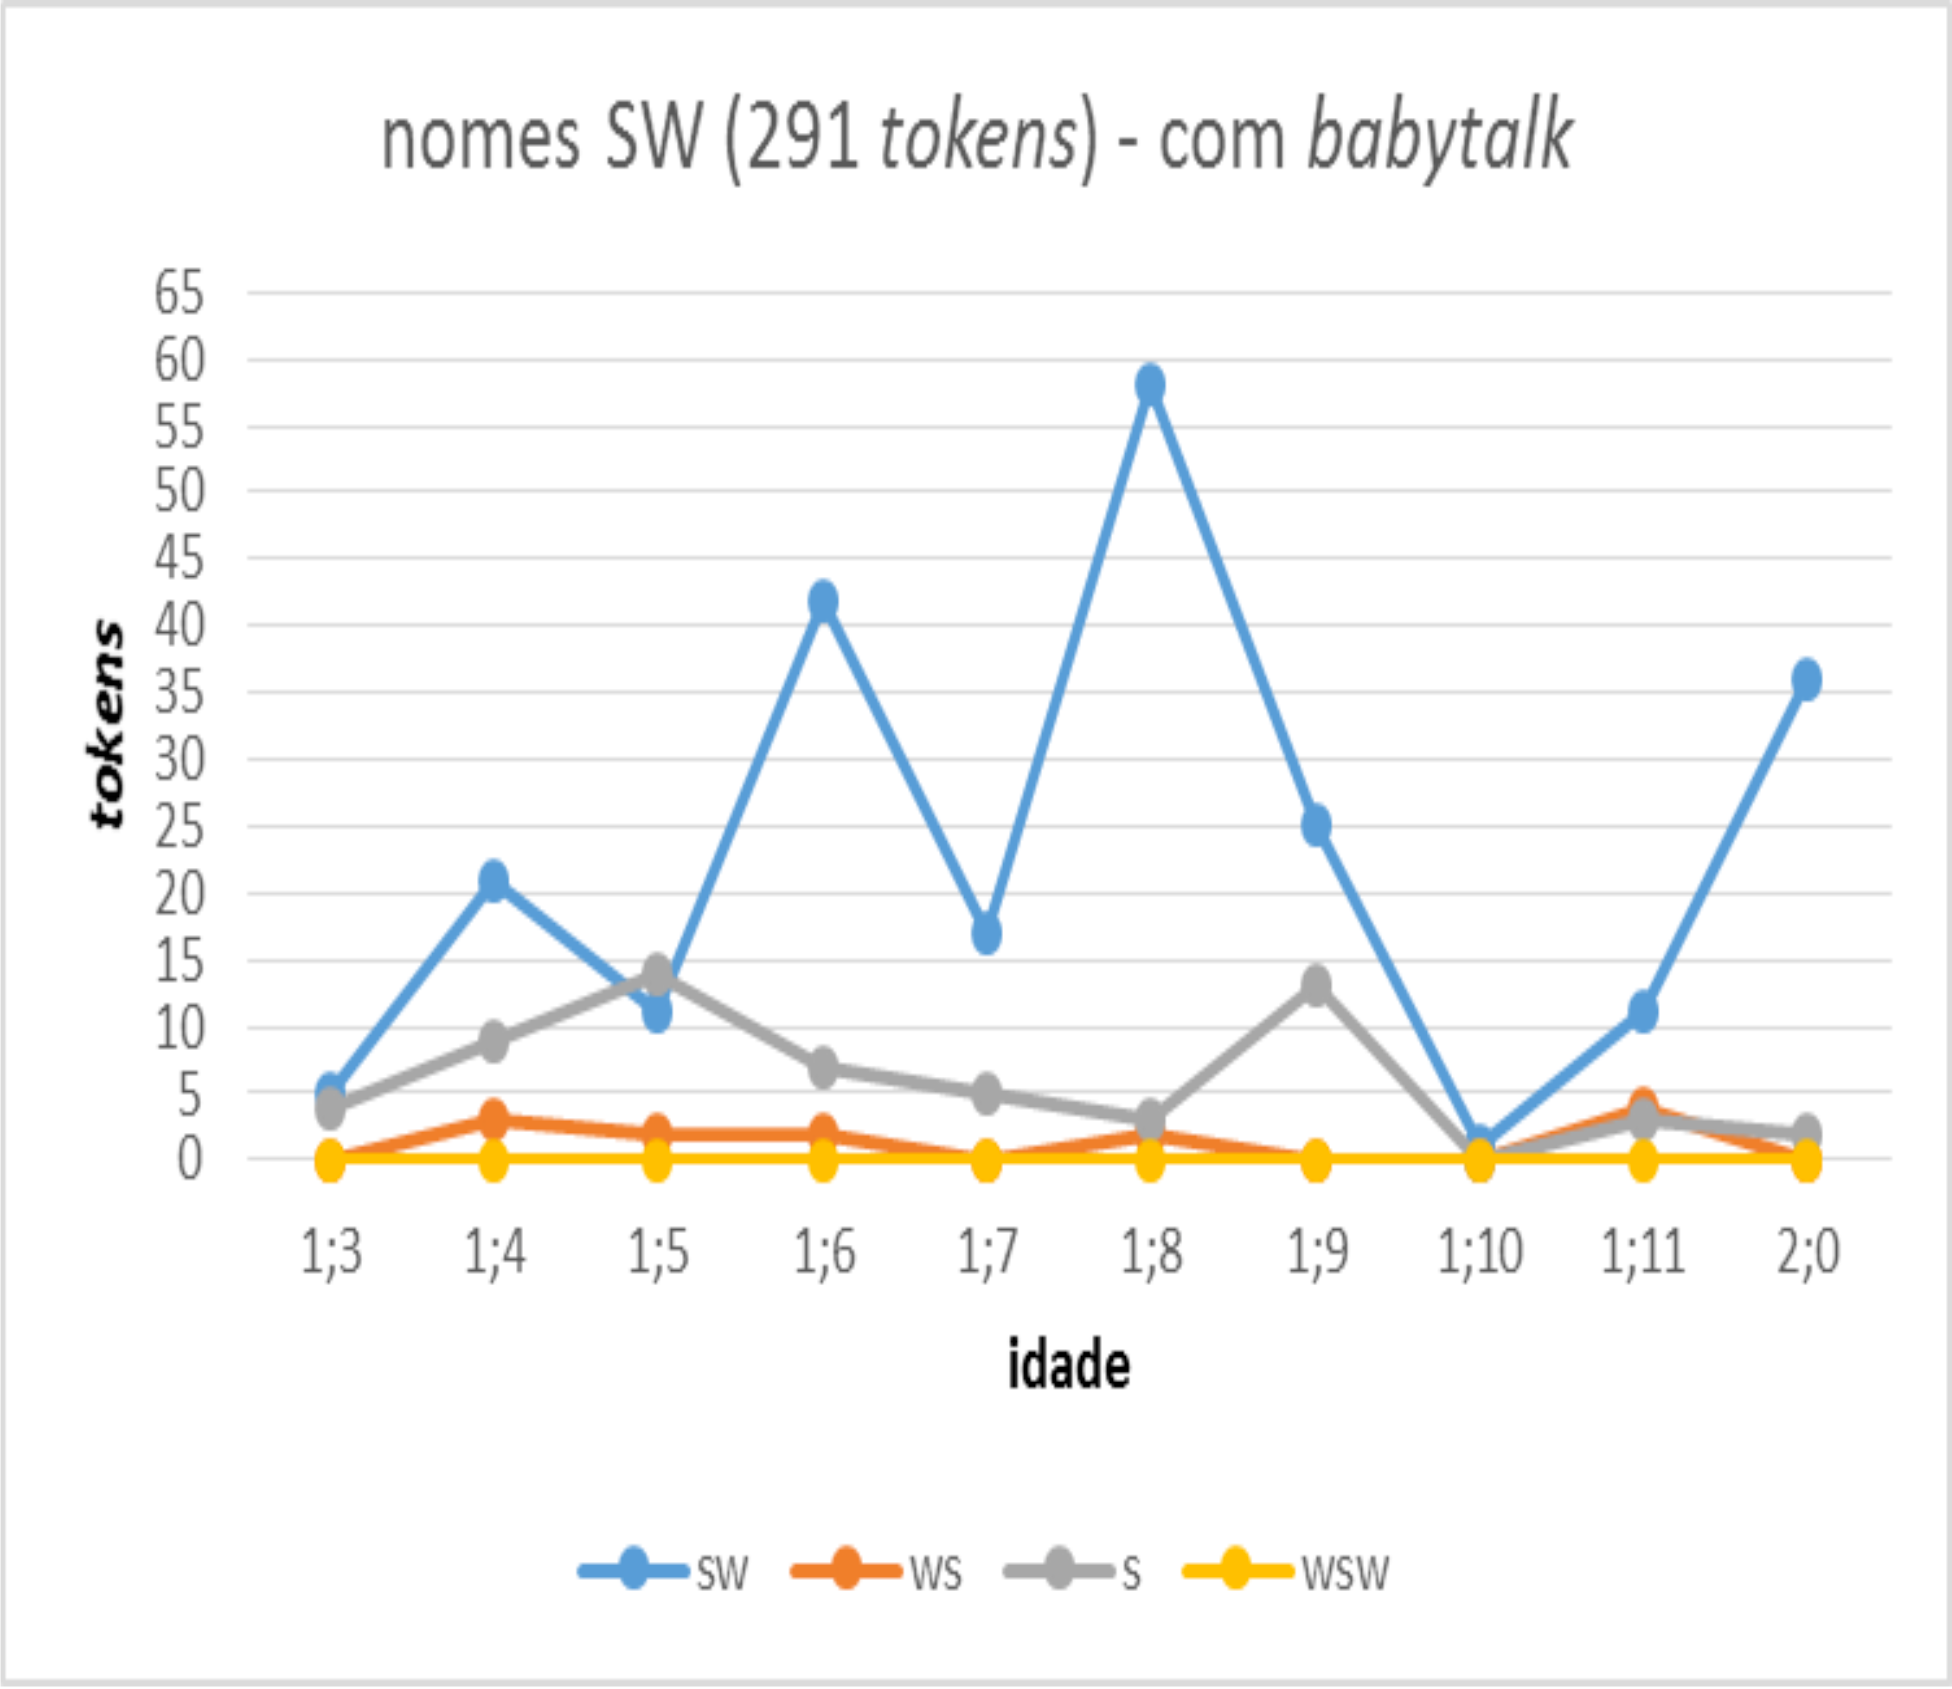
\includegraphics[width=0.5\textwidth]{figures/santanafig1}
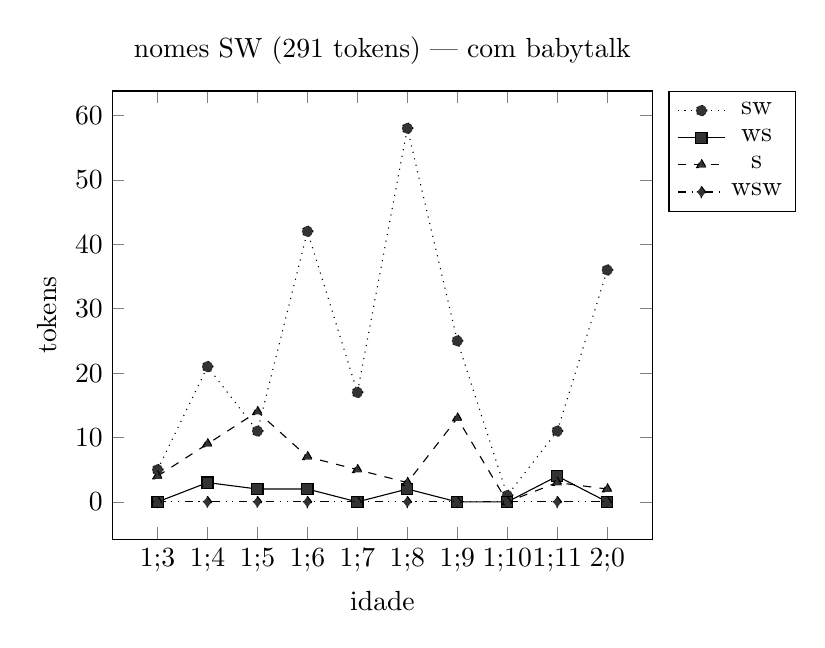
\begin{tikzpicture}
 \begin{axis}[legend pos=outer north east,symbolic x coords={1;3,1;4,1;5,1;6,1;7,1;8,1;9,1;10,1;11,2;0},ytick={0,10,...,60},xtick=data,xlabel=idade,ylabel=tokens,title=nomes SW (291 tokens) --- com babytalk]
  \addplot[black,dotted,mark=*,mark options={scale=1,fill=black!80}] table [x=RL, y=sw] {
  RL	sw
  1;3	5
  1;4	21
  1;5	11
  1;6	42
  1;7	17
  1;8	58
  1;9	25
  1;10	1
  1;11	11
  2;0	36
};
  \addplot[black,solid,mark=square*,mark options={scale=1,fill=black!80}] table[x=RL, y=ws] {
RL		ws
1;3		0
1;4		3
1;5		2
1;6		2
1;7		0
1;8		2
1;9		0
1;10		0
1;11		4
2;0		0
  };
  \addplot[black,dashed,mark=triangle*,mark options={scale=1,fill=black!80}] table[x=RL, y=s] {
 RL			s
1;3			4
1;4			9
1;5			14
1;6			7
1;7			5
1;8			3
1;9			13
1;10			0
1;11			3
2;0			2
  };
  \addplot[black, dashdotdotted,mark=diamond*,mark options={scale=1,fill=black!80}] table[x=RL, y=wsw] {
RL				wsw
1;3				0
1;4				0
1;5				0
1;6				0
1;7				0
1;8				0
1;9				0
1;10				0
1;11				0
2;0				0  
  };
  \legend{sw,ws,s,wsw};
 \end{axis}
\end{tikzpicture}
\caption{padrões prosódicos produzidos para nomes SW com palavras babytalk}
\label{fig:santana_1}
\end{figure}

\begin{figure}
% % 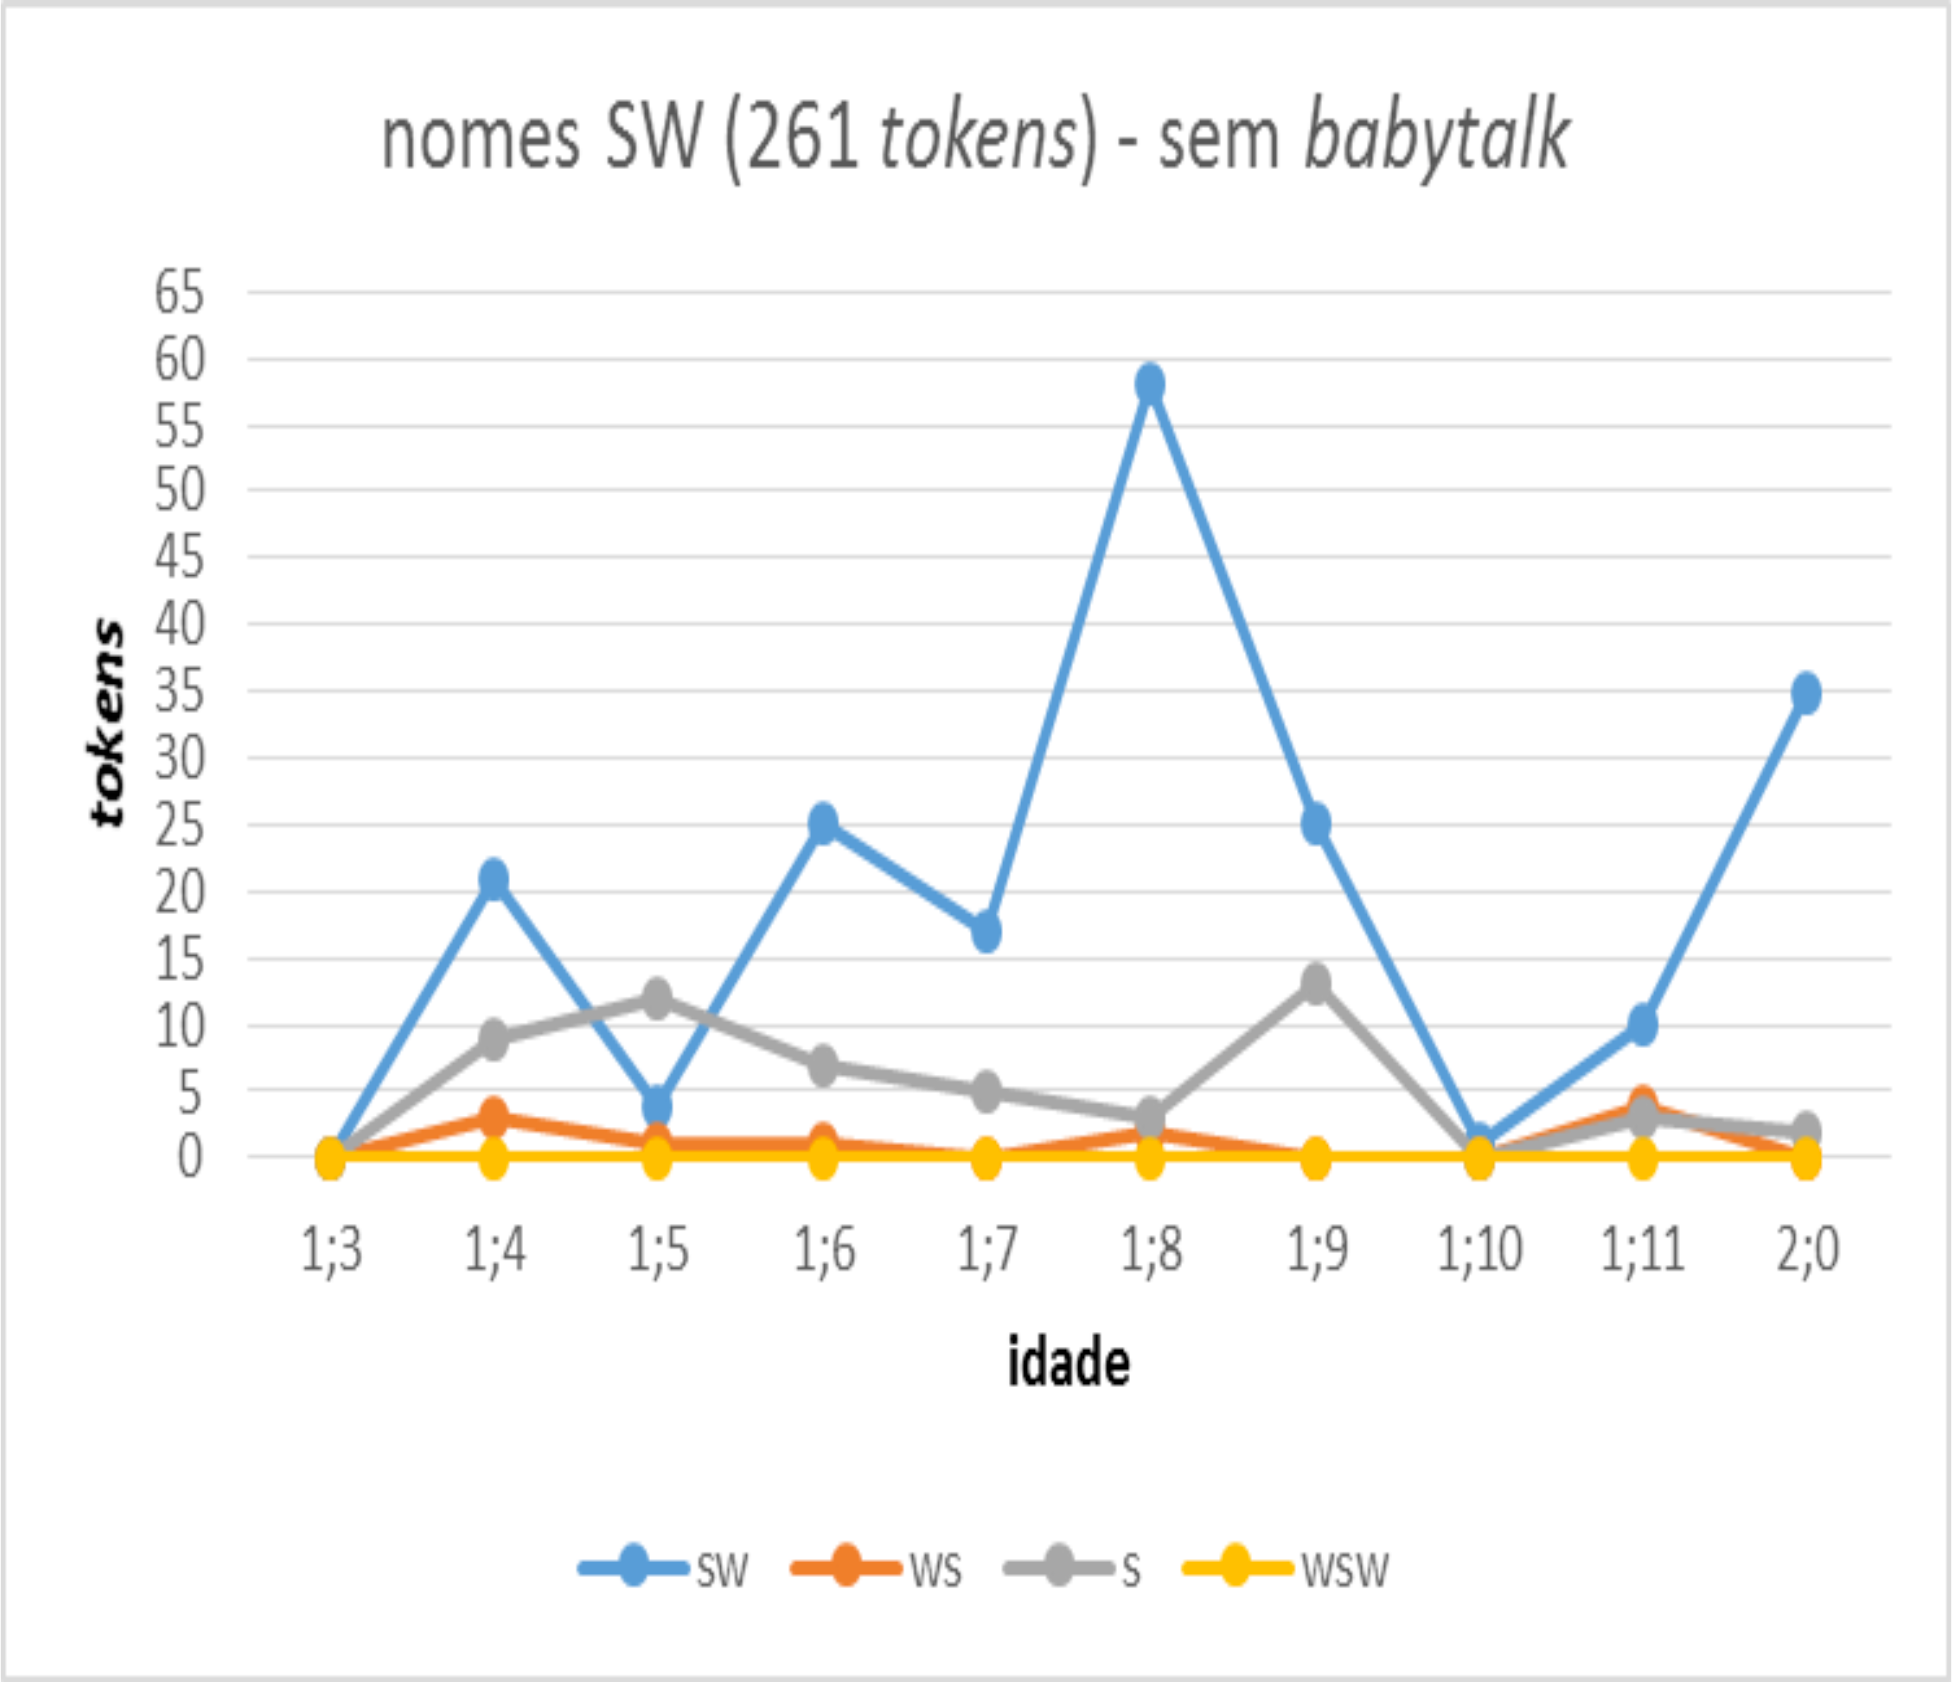
\includegraphics[width=0.5\textwidth]{figures/santanafig2}
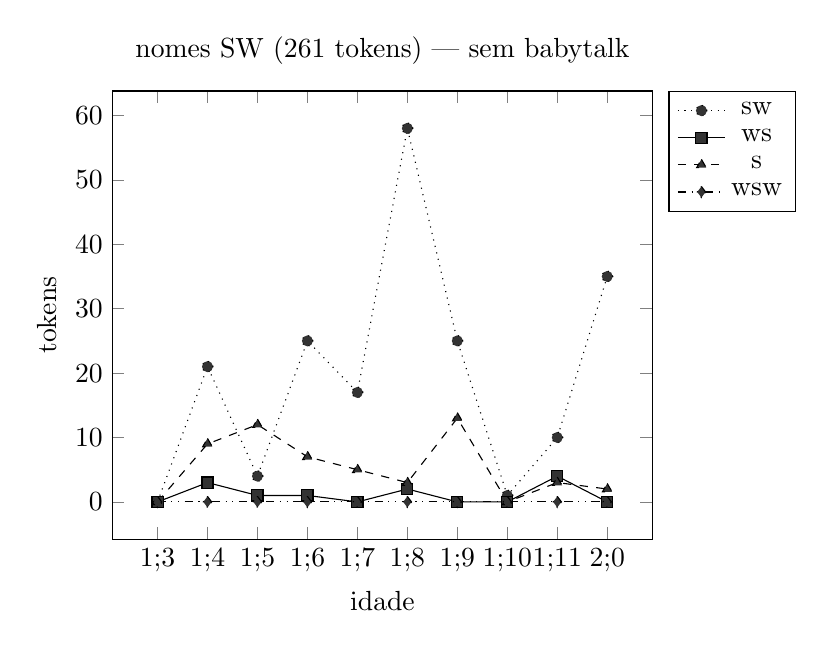
\begin{tikzpicture}
 \begin{axis}[legend pos=outer north east,symbolic x coords={1;3,1;4,1;5,1;6,1;7,1;8,1;9,1;10,1;11,2;0},ytick={0,10,...,60},xtick=data,xlabel=idade,ylabel=tokens,title=nomes SW (261 tokens) --- sem babytalk]
  \addplot[black,dotted,mark=*,mark options={scale=1,fill=black!80}] table [x=RL, y=sw] {
RL	sw
1;3	0
1;4	21
1;5	4
1;6	25
1;7	17
1;8	58
1;9	25
1;10	1
1;11	10
2;0	35
};
  \addplot[black,solid,mark=square*,mark options={scale=1,fill=black!80}] table[x=RL, y=ws] {
RL		ws
1;3		0
1;4		3
1;5		1
1;6		1
1;7		0
1;8		2
1;9		0
1;10		0
1;11		4
2;0		0
  };
  \addplot[black,dashed,mark=triangle*,mark options={scale=1,fill=black!80}] table[x=RL, y=s] {
RL			s
1;3			0
1;4			9
1;5			12
1;6			7
1;7			5
1;8			3
1;9			13
1;10			0
1;11			3
2;0			2
  };
  \addplot[black, dashdotdotted,mark=diamond*,mark options={scale=1,fill=black!80}] table[x=RL, y=wsw] {
RL				wsw
1;3				0
1;4				0
1;5				0
1;6				0
1;7				0
1;8				0
1;9				0
1;10				0
1;11				0
2;0				0 
  };
  \legend{sw,ws,s,wsw};
 \end{axis}
\end{tikzpicture}
\caption{padrões prosódicos produzidos para nomes SW sem palavras babytalk}
\label{fig:santana_2}
\end{figure}

As Figuras \ref{fig:santana_3} e \ref{fig:santana_4} apresentam a produção de padrões WS. O primeiro fato a se notar é a grande quantidade de palavras babytalk\is{babytalk@\textit{babytalk}} com esse padrão (somente 34 \textit{tokens} não eram \textit{babytalk}) (como `dodói' \ipa{[do\pstr dOj]}). Percebe-se algumas mudanças para um padrão SW (`gravador' como \ipa{[ga\pstr vado]}) em um período posterior ao da mudança de palavras SW para WS. A produção de iambos\is{padrão!iâmbico} como monossílabos também ocorre (WS produzidos como S) (`Miguel' como \ipa{[ge]}), principalmente em palavras do léxico adulto, e persiste por mais tempo.

\begin{figure}
% % 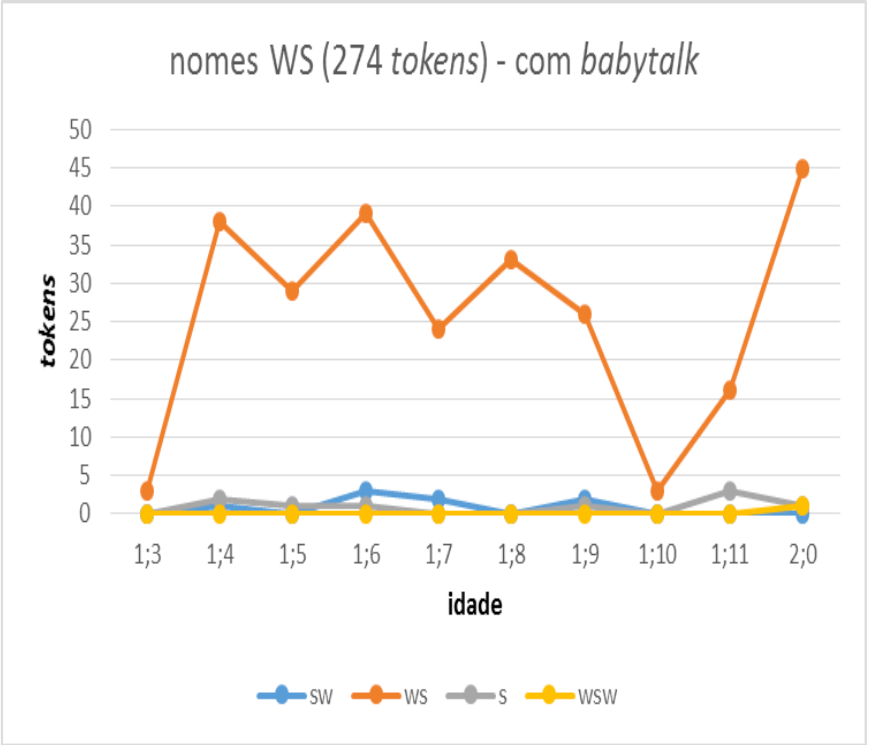
\includegraphics[width=0.5\textwidth]{figures/santanafig3}
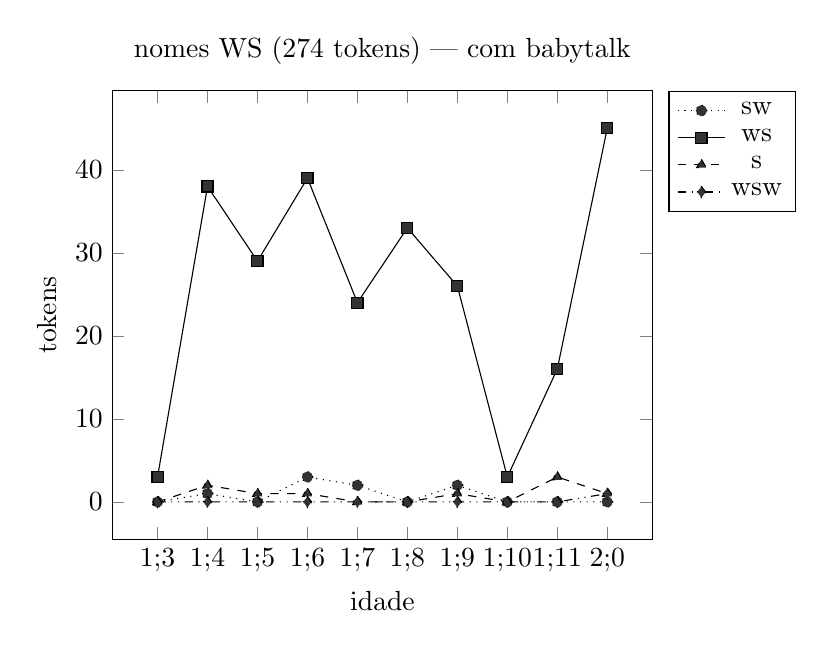
\begin{tikzpicture}
 \begin{axis}[legend pos=outer north east,symbolic x coords={1;3,1;4,1;5,1;6,1;7,1;8,1;9,1;10,1;11,2;0},ytick={0,10,...,60},xtick=data,xlabel=idade,ylabel=tokens,title=nomes WS (274 tokens) --- com babytalk]
  \addplot[black,dotted,mark=*,mark options={scale=1,fill=black!80}] table [x=RL, y=sw] {
RL	sw
1;3	0
1;4	1
1;5	0
1;6	3
1;7	2
1;8	0
1;9	2
1;10	0
1;11	0
2;0	0
};
  \addplot[black,solid,mark=square*,mark options={scale=1,fill=black!80}] table[x=RL, y=ws] {
RL		ws
1;3		3
1;4		38
1;5		29
1;6		39
1;7		24
1;8		33
1;9		26
1;10		3
1;11		16
2;0		45
  };
  \addplot[black,dashed,mark=triangle*,mark options={scale=1,fill=black!80}] table[x=RL, y=s] {
RL			s
1;3			0
1;4			2
1;5			1
1;6			1
1;7			0
1;8			0
1;9			1
1;10			0
1;11			3
2;0			1
  };
  \addplot[black, dashdotdotted,mark=diamond*,mark options={scale=1,fill=black!80}] table[x=RL, y=wsw] {
RL				wsw
1;3				0
1;4				0
1;5				0
1;6				0
1;7				0
1;8				0
1;9				0
1;10				0
1;11				0
2;0				1
  };
  \legend{sw,ws,s,wsw};
 \end{axis}
\end{tikzpicture}
\caption{padrões prosódicos produzidos para nomes WS com palavras babytalk}
\label{fig:santana_3}
\end{figure}

\begin{figure}
% % 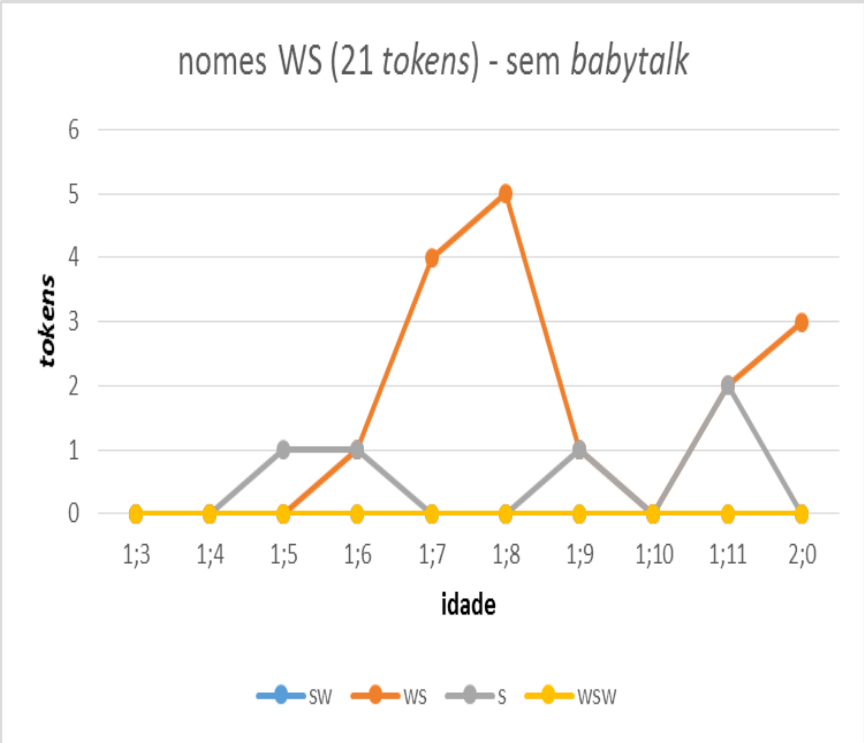
\includegraphics[width=0.5\textwidth]{figures/santanafig4}
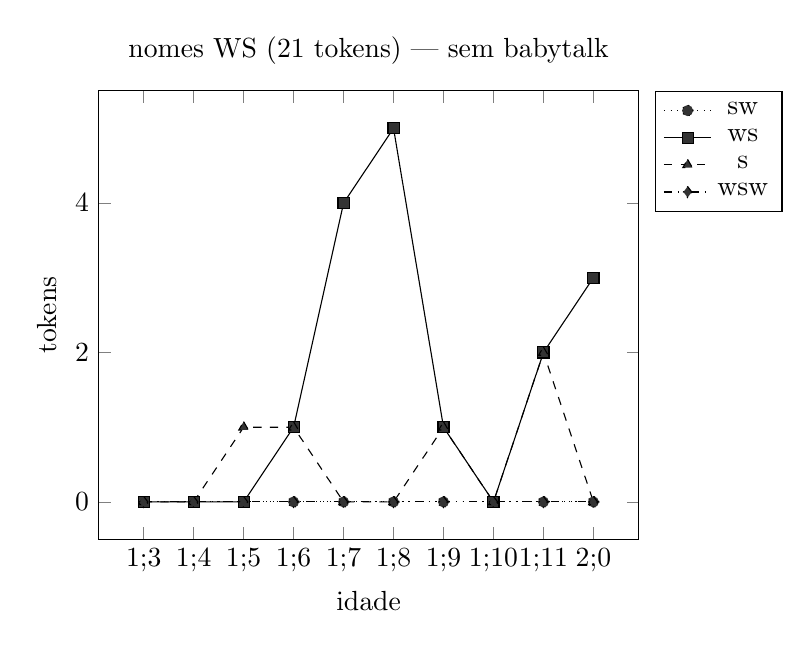
\begin{tikzpicture}
 \begin{axis}[legend pos=outer north east,symbolic x coords={1;3,1;4,1;5,1;6,1;7,1;8,1;9,1;10,1;11,2;0},ytick={0,2,...,60},xtick=data,xlabel=idade,ylabel=tokens,title=nomes WS (21 tokens) --- sem babytalk]
  \addplot[black,dotted,mark=*,mark options={scale=1,fill=black!80}] table [x=RL, y=sw] {
RL	sw
1;3	0
1;4	0
1;5	0
1;6	0
1;7	0
1;8	0
1;9	0
1;10	0
1;11	0
2;0	0
};
  \addplot[black,solid,mark=square*,mark options={scale=1,fill=black!80}] table[x=RL, y=ws] {
RL		ws
1;3		0
1;4		0
1;5		0
1;6		1
1;7		4
1;8		5
1;9		1
1;10		0
1;11		2
2;0		3
  };
  \addplot[black,dashed,mark=triangle*,mark options={scale=1,fill=black!80}] table[x=RL, y=s] {
RL			s
1;3			0
1;4			0
1;5			1
1;6			1
1;7			0
1;8			0
1;9			1
1;10			0
1;11			2
2;0			0
  };
  \addplot[black, dashdotdotted,mark=diamond*,mark options={scale=1,fill=black!80}] table[x=RL, y=wsw] {
RL				wsw
1;3				0
1;4				0
1;5				0
1;6				0
1;7				0
1;8				0
1;9				0
1;10				0
1;11				0
2;0				0
  };
  \legend{sw,ws,s,wsw};
 \end{axis}
\end{tikzpicture}
\caption{padrões prosódicos produzidos para nomes WS sem palavras babytalk}
\label{fig:santana_4}
\end{figure}

As Figuras \ref{fig:santana_5} e \ref{fig:santana_6} apresentam a produção de monossílabos. Como se pode perceber, são modificados para o padrão WS (`pé'\is{pé} como \ipa{[ti\pstr pa]}). Finalmente, o Figura \ref{fig:santana_7} traz as palavras com padrão WSW – não foi encontrada nenhuma palavra \textit{babytalk}\is{babytalk@\textit{babytalk}} nos dados. Embora trocaicas,\is{padrão!trocaico} estas palavras são analisadas separadamente porque, a depender de qual sílaba átona\is{sílaba!sílaba átona} a criança apaga, ela pode criar um padrão iâmbico\is{padrão!iâmbico} ou manter o padrão trocaico\is{padrão!trocaico} (mas com a palavra dissílaba).

\begin{figure}
% % 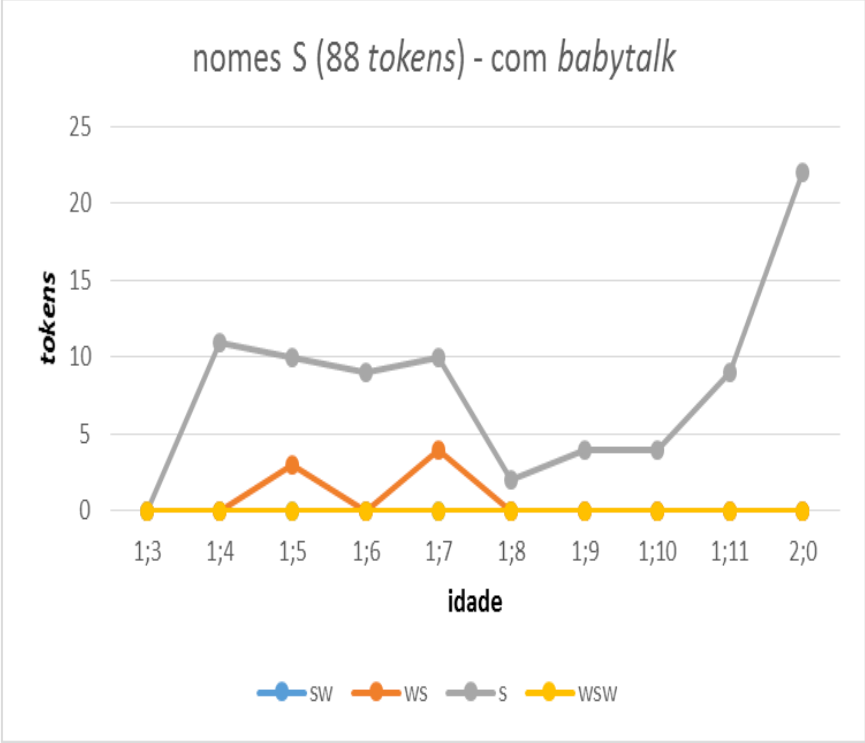
\includegraphics[width=0.5\textwidth]{figures/santanafig5} 
\caption{padrões prosódicos produzidos para nomes S com palavras babytalk}
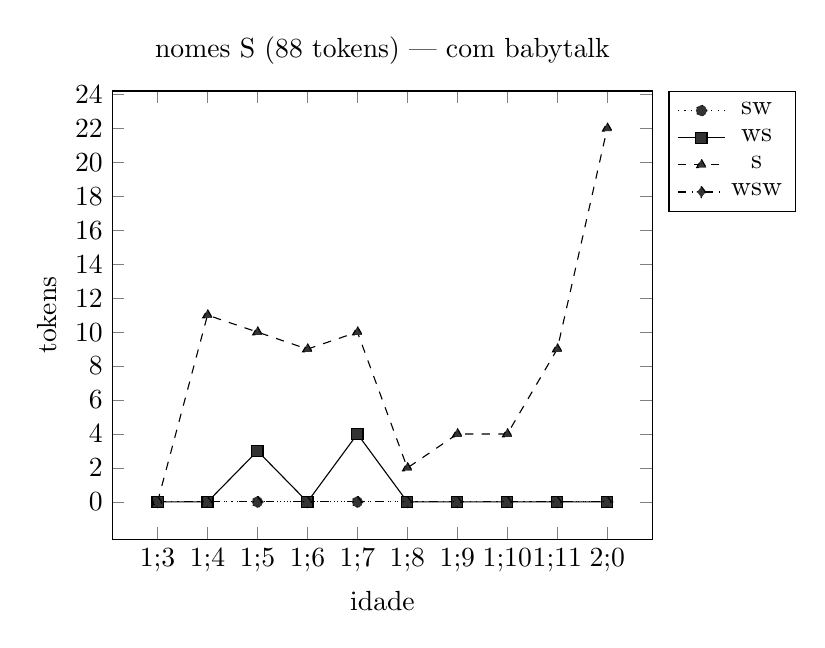
\begin{tikzpicture}
 \begin{axis}[legend pos=outer north east,symbolic x coords={1;3,1;4,1;5,1;6,1;7,1;8,1;9,1;10,1;11,2;0},ytick={0,2,...,60},xtick=data,xlabel=idade,ylabel=tokens,title=nomes S (88 tokens) --- com babytalk]
  \addplot[black,dotted,mark=*,mark options={scale=1,fill=black!80}] table [x=RL, y=sw] {
RL	sw
1;3	0
1;4	0
1;5	0
1;6	0
1;7	0
1;8	0
1;9	0
1;10	0
1;11	0
2;0	0
};
  \addplot[black,solid,mark=square*,mark options={scale=1,fill=black!80}] table[x=RL, y=ws] {
RL		ws
1;3		0
1;4		0
1;5		3
1;6		0
1;7		4
1;8		0
1;9		0
1;10		0
1;11		0
2;0		0
  };
  \addplot[black,dashed,mark=triangle*,mark options={scale=1,fill=black!80}] table[x=RL, y=s] {
RL			s
1;3			0
1;4			11
1;5			10
1;6			9
1;7			10
1;8			2
1;9			4
1;10			4
1;11			9
2;0			22
  };
  \addplot[black, dashdotdotted,mark=diamond*,mark options={scale=1,fill=black!80}] table[x=RL, y=wsw] {
RL				wsw
1;3				0
1;4				0
1;5				0
1;6				0
1;7				0
1;8				0
1;9				0
1;10				0
1;11				0
2;0				0
  };
  \legend{sw,ws,s,wsw};
 \end{axis}
\end{tikzpicture}
\label{fig:santana_5}
\end{figure}

\begin{figure}
% % 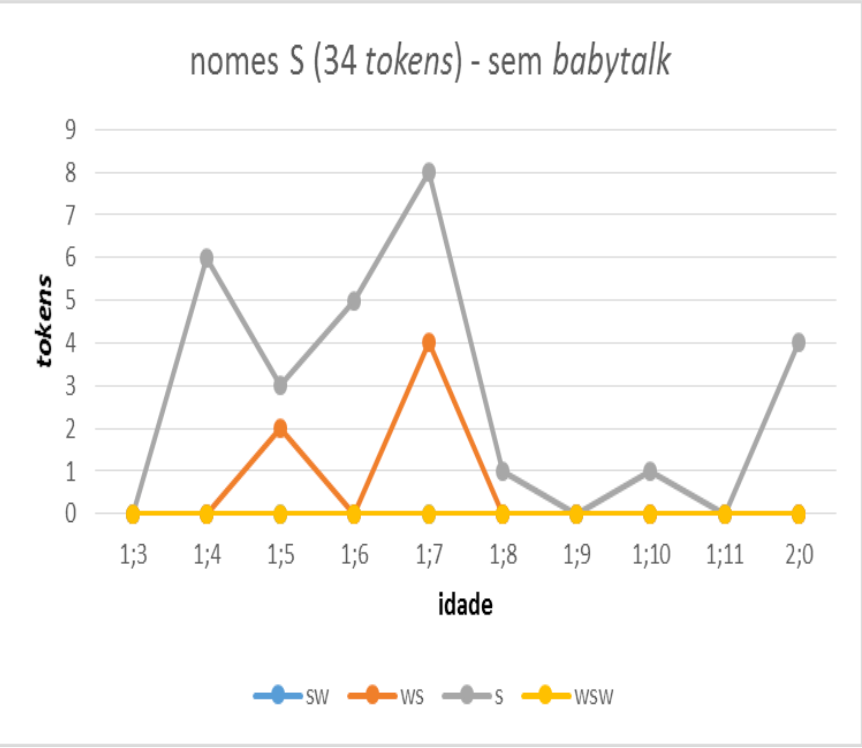
\includegraphics[width=0.5\textwidth]{figures/santanafig6}
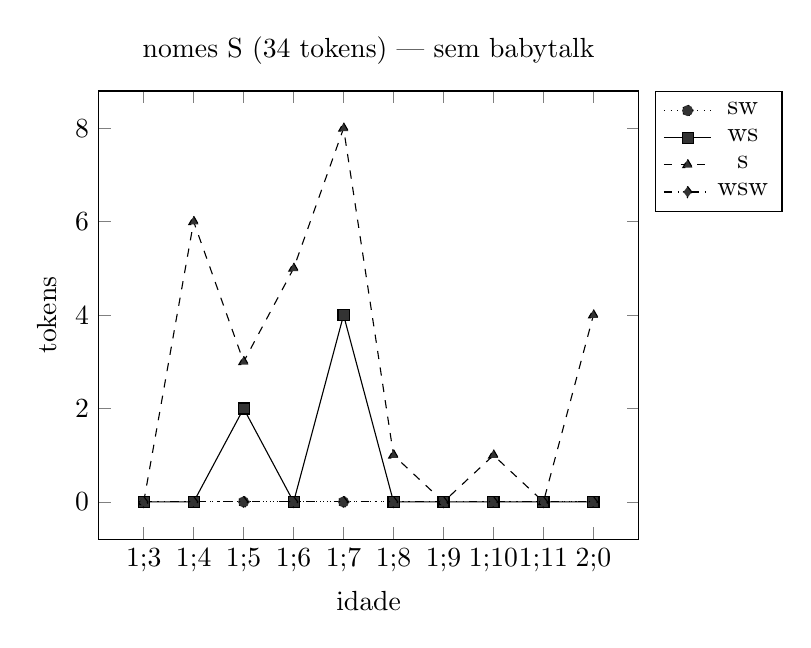
\begin{tikzpicture}
 \begin{axis}[legend pos=outer north east,symbolic x coords={1;3,1;4,1;5,1;6,1;7,1;8,1;9,1;10,1;11,2;0},ytick={0,2,...,60},xtick=data,xlabel=idade,ylabel=tokens,title=nomes S (34 tokens) --- sem babytalk]
  \addplot[black,dotted,mark=*,mark options={scale=1,fill=black!80}] table [x=RL, y=sw] {
RL	sw
1;3	0
1;4	0
1;5	0
1;6	0
1;7	0
1;8	0
1;9	0
1;10	0
1;11	0
2;0	0
};
  \addplot[black,solid,mark=square*,mark options={scale=1,fill=black!80}] table[x=RL, y=ws] {
RL		ws
1;3		0
1;4		0
1;5		2
1;6		0
1;7		4
1;8		0
1;9		0
1;10		0
1;11		0
2;0		0
  };
  \addplot[black,dashed,mark=triangle*,mark options={scale=1,fill=black!80}] table[x=RL, y=s] {
RL			s
1;3			0
1;4			6
1;5			3
1;6			5
1;7			8
1;8			1
1;9			0
1;10			1
1;11			0
2;0			4
  };
  \addplot[black, dashdotdotted,mark=diamond*,mark options={scale=1,fill=black!80}] table[x=RL, y=wsw] {
RL				wsw
1;3				0
1;4				0
1;5				0
1;6				0
1;7				0
1;8				0
1;9				0
1;10				0
1;11				0
2;0				0
  };
  \legend{sw,ws,s,wsw};
 \end{axis}
\end{tikzpicture}
\caption{padrões prosódicos produzidos para nomes S sem palavras babytalk}
\label{fig:santana_6}
\end{figure}

\begin{figure}
% % 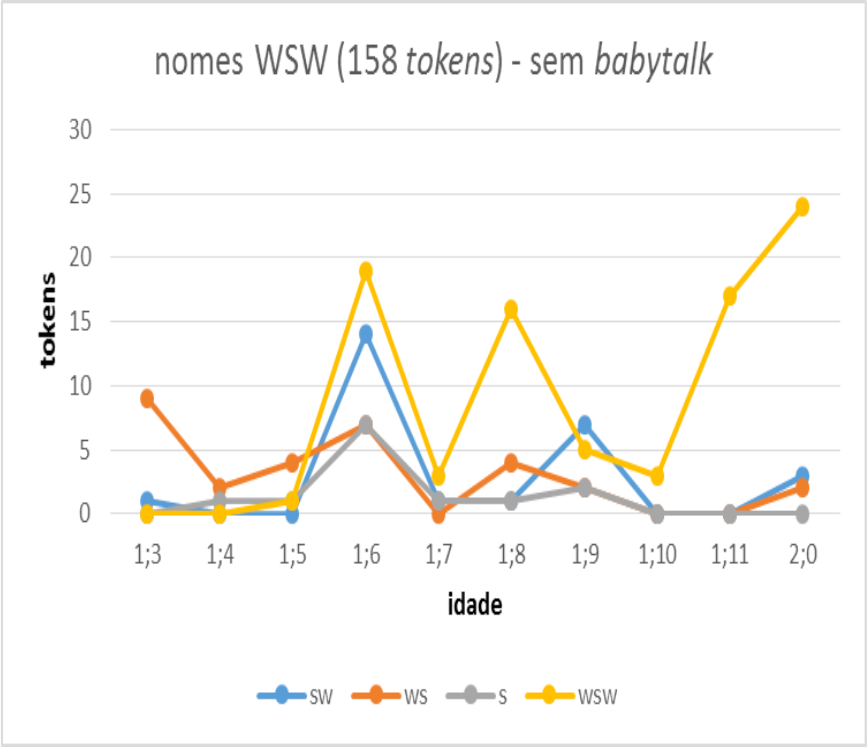
\includegraphics[width=0.5\textwidth]{figures/santanafig7} 
\caption{padrões prosódicos produzidos para nomes WSW sem palavras babytalk}
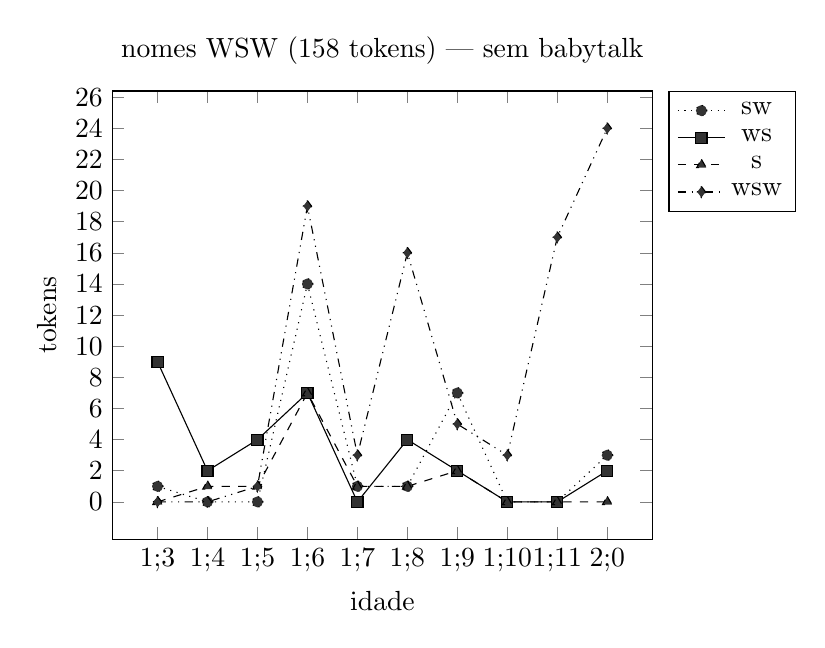
\begin{tikzpicture}
 \begin{axis}[legend pos=outer north east,symbolic x coords={1;3,1;4,1;5,1;6,1;7,1;8,1;9,1;10,1;11,2;0},ytick={0,2,...,60},xtick=data,xlabel=idade,ylabel=tokens,title=nomes WSW (158 tokens) --- sem babytalk]
  \addplot[black,dotted,mark=*,mark options={scale=1,fill=black!80}] table [x=RL, y=sw] {
RL	sw
1;3	1
1;4	0
1;5	0
1;6	14
1;7	1
1;8	1
1;9	7
1;10	0
1;11	0
2;0	3
};
  \addplot[black,solid,mark=square*,mark options={scale=1,fill=black!80}] table[x=RL, y=ws] {
RL		ws
1;3		9
1;4		2
1;5		4
1;6		7
1;7		0
1;8		4
1;9		2
1;10		0
1;11		0
2;0		2
  };
  \addplot[black,dashed,mark=triangle*,mark options={scale=1,fill=black!80}] table[x=RL, y=s] {
RL			s
1;3			0
1;4			1
1;5			1
1;6			7
1;7			1
1;8			1
1;9			2
1;10			0
1;11			0
2;0			0
  };
  \addplot[black, dashdotdotted,mark=diamond*,mark options={scale=1,fill=black!80}] table[x=RL, y=wsw] {
RL				wsw
1;3				0
1;4				0
1;5				1
1;6				19
1;7				3
1;8				16
1;9				5
1;10				3
1;11				17
2;0				24
  };
  \legend{sw,ws,s,wsw};
 \end{axis}
\end{tikzpicture}
\label{fig:santana_7}
\end{figure}

Em primeiro lugar, note-se que não há palavras infantis (\textit{babytalk})\is{babytalk@\textit{babytalk}} com padrão WSW. Em segundo lugar, essas palavras, nos primeiros meses (1;3-1;5), são modificadas para o padrão iâmbico\is{padrão!iâmbico} (`menino' como \ipa{[mi\pstr ni]}). Quando as crianças passam a modificar as palavras WSW para um padrão trocaico\is{padrão!trocaico} (`menino' como \ipa{[\pstr m\~{i}.\textltailn u]}), elas também já produzem o padrão alvo (`menino' como \ipa{[mi\pstr ni.nu]}), e em muito maior quantidade.
 Os gráficos também chamam a atenção para as diferentes estratégias que as crianças utilizam para a produção de um padrão prosódico:\is{padrão!prosódico} mudança no acento\is{acento} (cf. (\ref{ex:santana_7})), apagamento de sílabas (cf. (\ref{ex:santana_8})), inserção de sílabas (cf. (\ref{ex:santana_9})), e seleção de palavras (as crianças `preferem' produzir palavras com acento\is{acento} final – por isso a grande quantidade de \textit{babytalk}\is{babytalk@\textit{babytalk}} com padrão iâmbico,\is{padrão!iâmbico} por exemplo – ou as crianças evitam palavras com um determinado padrão – o que explicaria a quantidade menor de monossílabos). Cumpre também chamar a atenção de que as palavras reduplicadas\is{reduplicação} infantis (do \textit{babytalk}\is{babytalk@\textit{babytalk}} ou criadas pelas crianças) são em sua quase totalidade iâmbicas\is{padrão!iâmbico} (cf. (\ref{ex:santana_10})).
 
\ea\label{ex:santana_7}
música \ipa{[mu.\pstr zi.ka]}, gravador \ipa{[gra.\pstr va.dor]},  cansado \ipa{[k\~{a}.sa.\pstr du]}\\\jambox{\citep{santos2007}}
\z
\ea\label{ex:santana_8}
menino \ipa{[mi\pstr ni]} \ipa{[\pstr m\~{i}.\textltailn u]}, sapato \ipa{[pa\pstr pa]}, cavalo \ipa{[kaw\pstr a]}\\\jambox{\citep{santos2007}}
tomate \ipa{[\pstr mA.\lng do]}\jambox{\citep{correia2009}}
\z
\ea\label{ex:santana_9}
pé \ipa{[u\pstr pE]} \ipa{[ti\pstr pa]}, abre \ipa{[a.\pstr bej.a]}\jambox{\citep{santos2007}}
porta \ipa{[2\pstr do\lng]}, pão \ipa{[5\pstr p5]}, Bambi \ipa{[5\pstr b5]}\jambox{\citep{correia2009}}
\z
\ea\label{ex:santana_10}
cocô \ipa{[ko\pstr ko]}, dodói \ipa{[do\pstr dOj]} \ipa{[dO\pstr dOj]}, chapéu \ipa{[pa.pa\pstr paw]}\\\jambox{\citep{santos2007}}
mamãe \ipa{[m5.\pstr m\~{5}]}, sapato \ipa{[p5\pstr p5]}, laranja \ipa{[l5\pstr la\lng]}\\\jambox{\citep{vigario_etal2006}}
\z

Todos os trabalhos sobre o português (à exceção de \citealt{rapp1994}) concordam que a predominância do padrão iâmbico\is{padrão!iâmbico} ocorre apenas no início do processo de aquisição, sendo este depois suplantado pelo padrão trocaico.\is{padrão!trocaico} O exemplo (\ref{ex:santana_11}) ilustra esse percurso (exemplos de \citealt{santos2007}):

\ea\label{ex:santana_11}
\gllll menino {\ipa{[mi]} 1;4}\\
~ {\ipa{[me] [a\pstr mi] [mi\pstr mi]} 1;5}\\
~ {\ipa{[mi\pstr ni.nu]} 1;11}\\
~ {\ipa{[mi\pstr ni.nu] [\pstr mi.nu]} 2;0}\\
\z

Finalmente, algumas palavras devem ser ditas sobre a aquisição/domínio dos parâmetros\is{parâmetro} acústicos responsáveis pelo acento de palavra.\is{acento!de palavra} São ainda poucos os trabalhos sobre o assunto em português. \citet{frotavigario2008} descrevem o uso de acento\is{acento!nivelado} nivelado (\textit{level stress}) – por exemplo, `bola' produzido como \ipa{[\pstr pa.\pstr pa]} – e a \isi{retração acentual} – por exemplo, `bola' produzido como \ipa{[pa\pstr pa]} - no início do processo de aquisição. \citet{gamarossi1999} em um trabalho experimental com 2 crianças, refere que a criança de 4 anos já adquiriu a implementação da \isi{duração} para as sílabas tônicas, mas não para as sílabas átonas;\is{sílaba!sílaba átona} e que a criança de 4;9 anos está mais próxima do padrão adulto de \isi{duração} para as vogais, mas não para as consoantes, sílabas e palavras. \citet{correia2009} fez uma descrição detalhada da produção das primeiras palavras com crianças portuguesas. Os resultados mostram que no início do processo de aquisição não há controle sobre os parâmetros\is{parâmetro} acústicos pelas crianças. Ainda assim, os iambos\is{padrão!iâmbico} tenderam a ser produzidos com maiores valores de \isi{frequência fundamental}, \isi{intensidade} e \isi{duração}. Em um segundo momento, tanto iambos\is{padrão!iâmbico} quanto troqueus\is{padrão!trocaico} foram produzidos com maior \isi{proeminência} dos parâmetros\is{parâmetro} acústicos nas sílabas tônicas.
 
\section{A palavra prosódica}
\label{sec:santana_palavra_prosodica}

Ao falarmos sobre \isi{palavra prosódica}, a primeira coisa que devemos referir é que esta não se confunde com o que é palavra para outros componentes gramaticais, ou seja, não há necessariamente isomorfia entre o que é palavra para a sintaxe, para a morfologia e para a fonologia. Por exemplo, em (\ref{ex:santana_12}) temos uma palavra sintática (que preenche um nó sintático) mas que são duas palavras prosódicas. Em (\ref{ex:santana_13}) temos uma palavra morfológica que é analisada, em português, como duas palavras fonológicas:\footnote{Para maiores discussões, cf. \citealt{mateusdandrade2000}.}

\ea\label{ex:santana_12}
[João Maria]\textsubscript{sintagma nominal} [João]\textsubscript{palavra prosódica}\is{palavra prosódica} [Maria]\textsubscript{palavra prosódica}
\z
\ea\label{ex:santana_13}
[colherzinha]\textsubscript{palavra morfológica} [colher]\textsubscript{palavra prosódica} [zinha]\textsubscript{palavra prosódica}\is{palavra prosódica}
\z

O acento\is{acento} é uma das principais características da \isi{palavra prosódica}, pois as palavras têm mínima\footnote{Note-se, no entanto, que há uma pequena quantidade de palavras consideradas sem acento,\is{acento} os clíticos fonológicos.} e maximamente um acento\is{acento} (cf. \citealt{jakobson1941} sobre o caráter deliminativo do acento).\is{acento} Isto significa que um estrangeiro ou uma criança, sabendo desta propriedade, procura recortar uma sequência sonora em palavras obedecendo a este princípio, mas ainda assim poderá apresentar problemas na segmentação. Veja, por exemplo, que o verso abaixo em (14) pode ser recortado de diferentes formas em português brasileiro (indicamos 3 de 6 possibilidades):\footnote{Adaptação de verso da música Dada, de Gilberto Gil e Caetano Veloso, em álbum Tropicálica 2, 1993, gravadora WEA.}

\ea\label{ex:santana_14}\ipa{[a.\pstr dew.za.\pstr dew.za.fro.\pstr dZi.tS\i]}
\ea\label{ex:santana_14a}
A (para) Deus, a deusa Afrodite.
\ex\label{ex:santana_14b}
Adeus à deus Afrodite.
\ex\label{ex:santana_14c}
A deusa, a deus Afrodite
\zl

Além do acento,\is{acento} as palavras prosódicas apresentam características quanto a sua extensão e propriedades (segmentais e prosódicas).\footnote{A discussão sobre aquisição de segmentos e sílabas encontra-se no capítulo 3 deste volume; aqui só trataremos dos aspectos desta aquisição relevantes para a discussão da aquisição do \isi{acento} de palavra.} \citet{vigario2003} é um trabalho seminal na descrição das propriedades que identificam a \isi{palavra prosódica} em português: fenômenos relacionados às fronteiras de palavras (e.g. palavras em português não iniciam por \ipa{[\textltailn,R,L]}; vogais palatais não-altas são apagadas em final de \isi{palavra prosódica}: `passe' \ipa{[\pstr pas]} vs. `passemos' \ipa{[p5\pstr semuS]}), fenômenos que tomam a \isi{palavra prosódica} como domínio de ocorrência (e.g. o apagamento quando há duas palavras prosódicas: mono\sout{gamia} ou poligamia (mono)(gamia) ou (poli)(gamia) vs. *bio\sout{grafia} e discografia (biografia) e (discografia)) e fenômenos relacionados à \isi{proeminência} (e.g. apagamento de vogal átona em final de palavra se a palavra seguinte começa com uma vogal). 

\citet{vigario_etal2006} descrevem a distribuição dos diferentes tipos silábicos e quantidade de sílabas nas palavras na fala adulta do português europeu. Segundo os autores, as palavras distribuem-se da seguinte maneira, de acordo com sua extensão: monossílabos 19,8\%, dissílabos 42,6\%, trissílabos 18,4\%, polissílabos 7,6\%.\footnote{Em português brasileiro, \citet{cintra1997} aponta a seguinte distribuição: monossílabos 39,7\%, dissílabos 22\%, trissílabos 18,6\%, quatro sílabas 11\%, cinco ou mais sílabas 8,6\%. Observa-se novamente uma diferença na distribuição, principalmente entre os monossílabos e polissílabos, nas duas variedades de português.} Como se observa, a grande maioria é de dissílabos, e os monossílabos e trissílabos têm distribuição semelhante. Os tipos silábicos, por sua vez, distribuem-se diferentemente nas diversas posições das palavras. Por exemplo, sílabas com glides são mais frequentes em monossílabos. Como há propostas sobre o acento de palavra\is{acento!de palavra} que levam em conta a estrutura silábica, interessa-nos aqui duas estruturas silábicas: sílabas abertas\is{sílaba!sílaba aberta} (CV/V) e sílabas fechadas\is{sílaba!sílaba fechada} (CVC/CVG). As sílabas CV têm uma distribuição mais homogênea (Vigário et al. 2006): em posição inicial (11,56\%), interna (10,95\%), final (16,46\%) de palavra e em monossílabos (7,38\%). As sílabas V ocorrem muito mais em posição inicial (6,58\%) e em monossílabos (7,68\%) do que nas outras posições de palavra. As sílabas CVC, por outro lado, ocorrem muito mais em posição final (5,88\%) do que nas outras posições (e.g. inicial (2,52\%)). Finalmente, as sílabas CVG aparecem mais em posição inicial (0,87\%) e em monossílabos (0,82\%) do que em posição interna (0,45\%) ou em fim de palavra (0,52\%).

\section{A palavra prosódica nas produções infantis}
\label{sec:santana_palavra_prosodica_infantis}

Um dos primeiros estudos sobre aquisição da palavra prosódica no português\is{palavra prosódica} trata da fala \textit{babytalk}\is{babytalk@\textit{babytalk}} no português brasileiro \citep{stoelgammon1976}. Muitas das palavras são onomatopeicas, enquanto para outras também é possível identificar uma referência com a forma adulta (cf. (\ref{ex:santana_15}), (\ref{ex:santana_16}), mas (\ref{ex:santana_17})). São características destas palavras a \isi{reduplicação} (cf. (\ref{ex:santana_15})), a elisão de sílabas fracas\is{sílaba!sílaba fraca} (cf. (\ref{ex:santana_18})), bem como a assimilação (cf. (\ref{ex:santana_19})) e a simplificação de encontros consonantais (cf. (\ref{ex:santana_20})) (exemplos de \citealt{stoelgammon1976}):
\ea\label{ex:santana_15}\ipa{[uaw.aw]} cachorro\z
\ea\label{ex:santana_16}\ipa{[vo\pstr vo]} avô\z
\ea\label{ex:santana_17}\ipa{[pa\pstr pa]} comida, comer (também pai)\z
\ea\label{ex:santana_18}\ipa{[a.\pstr bo]} acabou\z
\ea\label{ex:santana_19}\ipa{[\pstr t\~{e}.te]} quente\z
\ea\label{ex:santana_20}\ipa{[fiw]} frio\z

\citeauthor{stoelgammon1976} mostra que a forma canônica destas palavras é CV.CV(V) e que, neste modelo, a consoante é quase sempre reduplicada\is{reduplicação} (frequentemente uma labial, dental ou alvéolo-palatal); no caso das vogais, a nasalização de uma vogal não é reduplicada,\is{reduplicação} e a \isi{proeminência} é majoritariamente final. O padrão identificado pela pesquisadora corrobora a proposta de \citet{demuth1996} de que, na aquisição da estrutura prosódica, há um período em que as palavras são minimamente dissilábicas (neste período, a palavra fonológica corresponderia a um \isi{pé} fonológico formado por duas sílabas simples CV). \citet{santos2001}, no entanto, chama a atenção de que a duplicação (quase majoritariamente da sílaba tônica, nos casos encontrados) não é um fenômeno muito comum em palavras que não \textit{babytalk}\is{babytalk@\textit{babytalk}} e que, nestes casos, nem pelo período em que ocorre, nem pela estrutura de palavra que cria, se aproximam da estrutura encontrada por \citeauthor{stoelgammon1976}. Veja que (\ref{ex:santana_21}) cria uma estrutura WWWS, (\ref{ex:santana_22}) uma estrutura WSW, (\ref{ex:santana_23}) uma estrutura WWSW, e (\ref{ex:santana_24}) uma estrutura WWWSW (exemplos de \citealt{santos2001}):

\ea\label{ex:santana_21}\ipa{[a.kor.do.\pstr ow]} acordou\z
\ea\label{ex:santana_22}\ipa{[xa.\pstr a.da]} roda\z
\ea\label{ex:santana_23}\ipa{[b\~{i}.ke.\pstr e.du]} brinquedo\z
\ea\label{ex:santana_24}\ipa{[za.a.ka.\pstr lE.E]} jacaré\z

De acordo com \citet{demuth1996}, o processo de aquisição da estrutura prosódica (e leia-se aqui de palavra) passa pelos seguintes estágios: (i) monossílabos CV; (ii) palavras mínimas, (iii) palavras com a extensão de um \isi{pé}; (iv) palavras com a extensão de 2 pés,\is{pé} (v) forma adulta. A diferença entre os estágios (ii) e (iii) é que, no estágio 2, a criança lida com a questão da quantidade silábica.\footnote{Em línguas que levam em conta a quantidade de palavra, uma sílaba pesada conta como 1 \isi{pé}.} Trata-se de um processo que vai dos níveis mais baixos aos mais altos da hierarquia prosódica. 

No entanto, algumas características destas primeiras palavras levam a uma interpretação de aquisição oposta à proposta de \citet{demuth1996}. A primeira característica é a emergência inicial do sistema entoacional\is{padrão!entoacional} da criança (cf. \citealt{gebara1984} e \citealt{frotavigario1994}). A segunda é o uso de um contorno entoacional\is{padrão!entoacional} completado por sons preenchedores\is{preenchedores prosódicos} (\textit{filler sounds})\is{filler sounds|see {preenchedores prosódicos}} quando a palavra não tinha sílabas suficientes para fazê-lo (cf. \citealt{scarpa1997}). Esta autora chama a atenção de que a criança usa um contorno - (L)L H* (L)\footnote{L indica tom baixo e H tom alto. No começo do processo, cada tom é associado a uma sílaba. Assim, L indica sílabas baixas e fracas,\is{sílaba!sílaba fraca} H sílabas altas, * sílaba portadora do acento entoacional,\is{acento!entoacional}\is{padrão!entoacional} os parênteses indicam opcionalidade. Assim, o padrão (L)L H*(L) indica um contorno de ao menos duas sílabas LH* (portanto um iambo),\is{padrão!iâmbico} podendo haver mais uma pré-tônica e uma pós-tônica.} – e alinha o acento de palavra\is{acento!de palavra} com o acento entoacional.\is{acento!entoacional}\is{padrão!entoacional} Baseada no fato de que, no começo do processo de aquisição, as estruturas sintáticas têm a extensão de uma palavra, \citet{santos2001} propõe que a criança ancora a produção de palavra (tanto em termos de quantidade de sílabas quanto de posição de \isi{proeminência}) no nível entoacional.\is{padrão!entoacional} Haveria um alinhamento entre a sílaba acentuada na palavra e o acento entoacional\is{acento!entoacional}\is{padrão!entoacional} (cf. (\ref{ex:santana_25})). As sílabas fracas\is{sílaba!sílaba fraca} seriam apagadas ou inseridas de forma a preencher este contorno entoacional\is{padrão!entoacional} (cf. (\ref{ex:santana_26}), (\ref{ex:santana_27})). \textit{Filler-sounds}\is{preenchedores de lugar} seriam utilizados quando a palavra alvo não tivesse tantas sílabas quanto as necessárias para preencher o contorno (cf. (\ref{ex:santana_28}), (\ref{ex:santana_29})). Poderia ser o caso de o acento de palavra\is{acento!de palavra} ser modificado para preencher o contorno entoacional\is{padrão!entoacional} (cf. (\ref{ex:santana_30})).

\begin{minipage}{\linewidth}% Following stays together
\begin{tabbing}
mmf. \= mm \= mmm \= mmm \= mmm \quad \= palavra \quad \= palavra \kill
~ \> (L) \> L \> H* \> (L) \> ~ \> ~
\end{tabbing}
\ea\label{ex:santana_25}
\begin{tabbing}
mm \= mmm \= mmm \= mmm \quad \= palavra \quad \= palavra \kill
~ \> si. \> ri \> ~ \> \ipa{[si.\pstr Ri]} \> siri
\end{tabbing}
\z
\ea\label{ex:santana_26}
\begin{tabbing}
mm \= mmm \= mmm \= mmm \quad \= palavra \quad \= palavra \kill
~ \> ~ \> mu. \> zi \> \ipa{[\pstr mu.zi]} \> música
\end{tabbing}
\z
\ea\label{ex:santana_27}
\begin{tabbing}
mm \= mmm \= mmm \= mmm \quad \= palavra \quad \= palavra \kill
~ \> ver. \> du \> ~ \> \ipa{[ver.\pstr du]} \> verdura
\end{tabbing}
\z
\ea\label{ex:santana_28}
\begin{tabbing}
mm \= mmm \= mmm \= mmm \quad \= palavra \quad \= palavra \kill
~ \> ~ \> maj. \> si \> \ipa{[\pstr mai.si]} \> mais
\end{tabbing}
\z
\ea\label{ex:santana_29}
\begin{tabbing}
mm \= mmm \= mmm \= mmm \quad \= palavra \quad \= palavra \kill
~ \> a. \> po \> ~ \> \ipa{[a.\pstr po]} \> por
\end{tabbing}
\z
\ea\label{ex:santana_30}
\begin{tabbing}
mm \= mmm \= mmm \= mmm \quad \= palavra \quad \= palavra \kill
~ \> mu. \> zi. \> ka \> \ipa{[mu.\pstr zi.ka]} \> música
\end{tabbing}
\z
~
\end{minipage}

\citet{frotavigario2008}, analisando acusticamente dados infantis do português europeu, propõem um processo de aquisição nas mesmas linhas, isto é, uma relação baseada no alinhamento entre o acento de palavra\is{acento!de palavra} e a entoação no início do processo de aquisição, em que as produções iniciais das crianças são ao mesmo tempo uma sílaba, uma \isi{palavra prosódica} e uma frase.

Tanto \citet{ferreiragoncalcesbrum2011} quanto \citet{baia2012} levantam a hipótese de que a frequência de padrões na língua alvo pode estar relacionada com a emergência do padrão de acento\is{acento} inicial com núcleo à direita (o iambo).\is{padrão!iâmbico} Segundo \citet{ferreiragoncalcesbrum2011}, a grande quantidade de iambos\is{padrão!iâmbico} no léxico adulto considerado frequente (25,6\% de oxítonos vs 23,1\% de paroxítonos) e possivelmente na fala dirigida à criança explicariam a quantidade de iambos\is{padrão!iâmbico} nas primeiras produções infantis. As autoras hipotetizam que a prevalência de iambos\is{padrão!iâmbico} no começo da aquisição seja devida à \isi{proeminência} psicolinguística de sílabas iniciais e de tônicas e à frequência de oxítonas no léxico. O padrão acentual\is{padrão!acentual} seria inicialmente rítmico, e sofreria modificações quando a morfologia fosse adquirida, havendo uma reanálise do \isi{pé} de acento.\is{acento} Veja que esta proposta não difere, em linhas gerais, da proposta de \citet{santos2001} exceto pelo fato de que, seguindo \citet{scarpa1997}, Santos propõe que a criança inicialmente começa pela curva entoacional\is{padrão!entoacional} e posteriormente reanalisa a estrutura em termos acentuais. Na Secção \ref{sec:santana_acento_pros_infantil}, veremos também que as crianças não seguem o padrão distribucional da fala que lhe é dirigida.

\citet{baia2012} propõe que a criança utiliza padrões fonológicos sistemáticos na aquisição do português (tanto no que diz respeito à quantidade de sílabas, estrutura silábica e posição de acento,\is{acento} bem como aspectos segmentais dos sons; por exemplo, os traços dos segmentos, que direcionariam a harmonia vocálica ou consonantal), o que facilitaria a expansão do léxico (cf. também \citealt{oliveiraguimaraes2012}). As principais diferenças de sua análise são as seguintes: a palavra é entendida como a unidade inicial com que a criança trabalha (os padrões seriam de palavra); estes padrões seriam vistos como estratégias individuais das crianças. Os resultados apontaram também para um início dissilábico com \isi{proeminência} final (ou seja, um iambo).\is{padrão!iâmbico}

Como temos chamado a atenção, inicialmente a produção infantil é dissilábica. Não é o caso de que não surjam monossílabos, mas eles não são em quantidade significativamente menor do que os padrões dissilábicos. Os resultados de uma das crianças estudadas por \citet{correia2009} ilustram a questão: Inês produz na primeira sessão 11 WS contra 3 S.  Segundo a autora, a grande quantidade de dissílabos iâmbicos\is{padrão!iâmbico} nas primeiras produções se deve às estratégias de duplicação e epêntese e ela questiona se estas produções devem ser interpretadas como iâmbicas\is{padrão!iâmbico} já que, nesta faixa etária, a criança não domina os parâmetros\is{parâmetro} acústicos de acento primário\is{acento!primário} (cf. também \citealt{gamarossi1999}). Uma questão que merece ser mais aprofundada é se, para se defender a aplicação de um algoritmo, deve-se também assumir que as crianças dominem princípios acústicos característicos do domínio (neste caso, a palavra), ou o algoritmo e os parâmetros\is{parâmetro} acústicos podem ser adquiridos de forma independente. \citet{santos2001} e \citet{frotavigario2008} seguem na segunda direção, hipotetizando que a criança utiliza o acento entoacional\is{acento!entoacional}\is{padrão!entoacional} como marcador de \isi{proeminência} de palavra.

\section{Acento e palavra prosódica: uma análise sobre a produção infantil}
\label{sec:santana_acento_pros_infantil}

Como vimos, no início do processo de aquisição as crianças apresentam mais palavras com padrão iâmbico\is{padrão!iâmbico} do que com padrão trocaico.\is{padrão!trocaico}\is{padrão!troqueu|see {padrão!trocaico}} Tal fato torna o português muito interessante para a discussão sobre aquisição de acento\is{acento} por dois motivos: o padrão iâmbico\is{padrão!iâmbico}\is{padrão!jâmbico|see {padrão!iâmbico}} inicial aparece em uma língua que tem padrão trocaico\is{padrão!trocaico} na fala adulta; o padrão iâmbico\is{padrão!iâmbico} inicial põe em cheque a proposta de uma tendência trocaica\is{padrão!trocaico} universal.

A análise de \citet{santos2001} e de \citet{frotavigario2008} propõem que este padrão ocorre porque a criança está utilizando o acento entoacional\is{acento!entoacional}\is{padrão!entoacional} como acento de palavra.\is{acento!de palavra} No entanto, isto não é suficiente para explicar o padrão iâmbico,\is{padrão!iâmbico} dado que, se é um fato que o acento entoacional\is{acento!entoacional}\is{padrão!entoacional} recai mais à direita nas estruturas sintáticas, não é verdade que ele recai sobre a última sílaba da estrutura. O exemplo (\ref{ex:santana_27}) acima ilustra a questão: a criança teria uma sílaba fraca\is{sílaba!sílaba fraca} final opcional para produzir \textit{verdura}. Por que não o faz? E por que o padrão iâmbico\is{padrão!iâmbico}\largerpage é preferido em relação ao padrão trocaico?\is{padrão!trocaico}

\citet{santos2007} investiga várias hipóteses, e seus resultados para uma das crianças analisadas – L. -  são reportados abaixo para ilustrar a discussão.\footnote{Cumpre chamar a atenção para uma questão metodológica: a autora só considerou para análise palavras que ocorressem mais de 8 vezes ao longo do período analisado (1;3 a 2;0) e não levou em conta palavras \textit{babytalk}\is{babytalk@\textit{babytalk}} ou criadas por \isi{reduplicação}. Assim, palavras como `pé',\is{pé} por exemplo, que fazem parte do vocabulário infantil, acabaram não fazendo parte da análise porque não apareceram o mínimo de vezes estabelecido, e palavras como `auau' para `cachorro' foram desconsideradas por serem criadas por um fenômeno que privilegia iambos.}\is{padrão!iâmbico} A distribuição dos padrões prosódicos\is{padrão!prosódico} variava conforme se somasse nomes e verbos ou os analisasse separadamente, e se levava em conta ou não as palavras infantis, \textit{babytalk}.\is{babytalk@\textit{babytalk}} O padrão geral encontrado (verbos e nomes, com palavras \textit{babytalk})\is{babytalk@\textit{babytalk}} foi 42,6\% de WS, 42\% de SW e WSW, e 15,4\% de monossílabos.


A primeira hipótese verificada foi se seria possível creditar a emergência mais inicial do padrão iâmbico\is{padrão!iâmbico} à frequência do \textit{input}. Para isso, é necessário ter em conta que falamos de forma diferente com as crianças, usando \textit{babytalk},\is{babytalk@\textit{babytalk}} palavras no diminutivo, o que em princípio pode modificar a distribuição dos padrões prosódicos\is{padrão!prosódico} a que a criança tem acesso. Feita uma comparação entre a distribuição do padrão acentual\is{padrão!acentual} na fala adulta e na fala dirigida à criança, confirmou-se, estatisticamente, uma diferente distribuição entre os padrões acentuais nas duas amostras. No entanto, a grande diferença não reside na maior quantidade de palavras com acento\is{acento} final mas em maior quantidade de monossílabos. Na fala dirigida a L., por exemplo, os iambos\is{padrão!iâmbico} somaram 19,50\% (contra 19,35\% na fala adulta) e os monossílabos somaram 21,22\% (contra 13,37\% na fala adulta). As palavras com acento\is{acento} na penúltima sílaba estão em menor quantidade, mas ainda assim são a maioria (na fala adulta, 67,28\%, na fala dirigida à criança, 59,28\%), o que não explica, portanto, a produção iâmbica\is{padrão!iâmbico} inicial.

Face a esse resultado, a autora observa se a produção da criança reflete a produção da fala que lhe é dirigida. 42,60\% das palavras que L. tentou produzir eram WS, enquanto ela só escutou 19,50\% desse padrão. SW e WSW somavam 59,28\% na fala dirigida, e L. tentou produzir palavras com este padrão 41,97\%. Finalmente, na fala dirigida os monossílabos somavam 21,22\%, mas L. só tentou produzir 15,42\% de palavras monossílabas. Em suma, o que L. tenta produzir não se assemelha à distribuição dos padrões prosódicos\is{padrão!prosódico} que ela escuta.

A autora também compara a distribuição dos padrões prosódicos\is{padrão!prosódico} da forma alvo das palavras produzidas pelas crianças e a sua efetiva produção para observar que tipo de forma alvo está sendo modificada. Isto é, a maior quantidade de monossílabos encontrada na fala das crianças (20,85\% na fala infantil vs. 13,37\% na fala adulta) origina-se de que tipo de palavra da forma alvo? Para todos os padrões prosódicos\is{padrão!prosódico} encontrou-se uma diferença significativa entre a forma alvo e a forma produzida. Como para estas análises as palavras \textit{babytalk}\is{babytalk@\textit{babytalk}} poderiam interferir nos resultados (já que são majoritariamente oxítonas), a autora levou em conta a distribuição prosódica somente dos nomes, sem \textit{babytalk}.\is{babytalk@\textit{babytalk}} Os resultados apontaram que L. selecionou 5,53\% de palavras com acento final,\is{acento} mas produziu 11,06\% do seu \textit{corpus} com acento final.\is{acento} Por outro lado, 94,47\% das palavras que L. tentou produzir eram na fala adulta troqueus,\is{padrão!trocaico} mas L. produziu em seu \textit{corpus} apenas 68.09\% de troqueus.\is{padrão!trocaico} L. não tentou produzir nenhuma palavra alvo monossílaba, mas produziu 20,85\% de palavras com formato monossílabo. Em linhas gerais, as crianças produziram mais iambos\is{padrão!iâmbico} e monossílabos do que era esperado pela seleção das palavras na fala adulta. Ainda assim, a quantidade de troqueus\is{padrão!trocaico} produzidos foi maior do que a de iambos.\is{padrão!iâmbico} O problema se coloca quando se observa a distribuição dos padrões ao longo do tempo, pois como vimos nas Figuras da Secção \ref{sec:santana_producoes_infantis}, os iambos\is{padrão!iâmbico} estão concentrados no começo do processo de aquisição.

Uma outra hipótese é a seguinte: a criança está evitando selecionar alguns padrões prosódicos\is{padrão!prosódico} para a produção. Neste caso, as crianças escolheriam outras estruturas – como se estivessem selecionando sinônimos. Por exemplo, no início da produção a criança preferiria dizer `guri' (WS) a `menino' (WSW), já que `guri' é uma dissílaba e `menino' uma trissílaba, um tamanho de palavra que ela ainda não dominaria. Os resultados mostraram que este não é o caso, as crianças não estão selecionando as palavras alvo a depender do padrão prosódico\is{padrão!prosódico} da mesma. Embora L. produza muitos iambos,\is{padrão!iâmbico} isso não se deve ao fato de que ela só escolhe palavras iâmbicas\is{padrão!iâmbico} na forma adulta. De fato, 64\% do léxico de L. é de palavras que são trocaicas\is{padrão!trocaico} (SW e WSW) na forma adulta. Palavras alvo monossilábicas e iâmbicas\is{padrão!iâmbico} também são selecionadas para produção (12,96\% e 23,02\%, respectivamente).

São analisadas, então, duas hipóteses de base mais linguística. A proposta de que a aquisição da forma prosódica obedece a um percurso dos níveis mais baixos (sílaba, \isi{pé}, palavra) para os mais altos (frase entoacional)\is{padrão!entoacional} na hierarquia prosódica também não parece ser sustentada pelos dados, levando-se em conta as análises de \citet{santos2001} e de \citet{frotavigario2008} de que, inicialmente, há uma influência do contorno entoacional\is{padrão!entoacional} na palavra. Além do mais, propostas de aquisição deste tipo acabam por apresentar um problema interno à própria teoria prosódica. Estas propostas de aquisição, em sua grande maioria, assumem que um dos primeiros estágios das palavras infantis é aquele em que a palavra tem o tamanho de 1 \isi{pé} (uma unidade de duas sílabas), com núcleo à esquerda – portanto, uma palavra SW (cf. Secção \ref{sec:santana_palavra_prosodica}). No entanto, de acordo com as versões mais difundidas de Teoria Prosódica, a posição do núcleo do \isi{pé} é estabelecida de acordo com cada língua específica. Em outras palavras, o \isi{pé} é universal, mas a posição do núcleo não -  logo, não deveríamos encontrar uma tendência diferente da tendência da língua alvo na fala das crianças. Assim, as explicações sobre a estrutura prosódica das primeiras palavras baseadas na hierarquia prosódica não explicam a emergência do iambo\is{padrão!iâmbico} no início do processo de aquisição do português.

Finalmente, há propostas calcadas na aquisição do algoritmo de acentuação. \citet{fikkert1994} é a principal referência para este tipo de trabalho. A proposta de \citeauthor{fikkert1994} insere-se dentro de uma visão paramétrica de aquisição. Segundo a autora, a posição do núcleo do \isi{pé} seria um \isi{parâmetro} a ser marcado e este \isi{parâmetro} teria um valor \textit{default} à esquerda (portanto, um SW). Caso a criança esteja adquirindo uma língua cuja forma alvo é SW (como é o caso do holandês),\il{holandês} a criança mantém o \isi{parâmetro} com o valor \textit{default}. Caso a criança adquira uma língua que na forma alvo é um iambo\is{padrão!iâmbico} (WS), ela deve trocar o valor do \isi{parâmetro} de núcleo à esquerda para núcleo à direita. Crucialmente, a criança só faz esta mudança quando compara a sua produção com a forma adulta. Isto significa que as primeiras produções infantis vão obedecer aos valores \textit{default} dos parâmetros.\is{parâmetro}

Vejamos como essa proposta se aplica aos dados. Se o valor \textit{default} do \isi{parâmetro} é núcleo à esquerda (SW), então se uma criança está adquirindo uma língua também SW, ela nunca cometerá erros. E foi o que \citeauthor{fikkert1994} encontrou. No entanto, essa proposta falha para explicar os dados do português, porque as crianças brasileiras e portuguesas apresentaram um padrão WS no começo, e não um padrão SW. Se alterarmos a proposta de \citeauthor{fikkert1994} de que o valor \textit{default} do \isi{parâmetro} de núcleo é esquerdo e postularmos que é direito, agora o que se espera é que as crianças comecem produzindo WS, mesmo em línguas cujo padrão adulto seja SW. Agora explica-se os dados encontrados para o português, mas cria-se um problema para o holandês,\il{holandês} já que \citeauthor{fikkert1994} não encontrou essa tendência de palavras WS no começo do processo de aquisição.

Esta parece ser então mais uma tentativa fracassada de explicar os iambos\is{padrão!iâmbico} iniciais, mas não necessariamente. As propostas de aquisição via marcação de parâmetros\is{parâmetro} podem ser divididas em duas: aquelas que assumem que os parâmetros\is{parâmetro} têm um valor inicial (\textit{default}) e aquelas que defendem que os parâmetros\is{parâmetro} não vêm com um valor marcado, apenas com as possibilidades de marcação, e é só frente ao \textit{input} que a escolha será feita. Assumindo-se um \isi{parâmetro} de núcleo com duas \textit{possibilidades} (direita (WS) e esquerda (SW)) sem valor \textit{default} e que a criança só pode começar a produzir dissílabos quando este \isi{parâmetro} estiver marcado (já que as palavras devem ter uma \isi{proeminência}), não será possível produções com um valor diferente do da língua alvo. Assim, as crianças adquirindo inglês\il{inglês} e holandês\il{holandês} produzem inicialmente troqueus\is{padrão!trocaico} porque este já o padrão da língua alvo,\largerpage e as crianças portuguesas e brasileiras produzem inicialmente iambos\is{padrão!iâmbico} porque este é o padrão do português. 

Mas cumpre lembrar que há no português adulto muito mais palavras paroxítonas do que oxítonas. Como explicar que as crianças produzam esse padrão prosódico?\is{padrão!prosódico} Se lembrarmos de nossa discussão sobre o algoritmo de acento\is{acento} na Secção \ref{sec:santana_acento}, vimos que a proposta de Lee é que o acento\is{acento} se deve à atribuição de um constituinte binário com núcleo à direita na palavra, mas ignorando o morfema marcador de palavra (cf. (\ref{ex:santana_2}) na Secção \ref{sec:santana_producoes_infantis}). Oras, se observarmos as palavras \textit{babytalk},\is{babytalk@\textit{babytalk}} que fazem parte do \textit{input} infantil, veremos que elas não têm esse morfema. O par mínimo em (\ref{ex:santana_31}) ilustra este ponto. `Cocô' é \textit{babytalk}\is{babytalk@\textit{babytalk}} e não apresenta marcador de palavra (veja que o [o] final não pode ser apagado na palavra derivada em (\ref{ex:santana_31a}), ao contrário da palavra derivada de `coco' em (\ref{ex:santana_31b})):

\ea\label{ex:santana_31}
\ea\label{ex:santana_31a}
\glll {cocô} > cocozada (*cocada) `A criança está toda cocozada.'\\
{(w~s)}\\
cocô\\
\ex\label{ex:santana_31b}
\glll coco > cocada (*cocozada) `Eu comi uma cocada.'\\
{(ws)}\\
coc[o]\\
\zl

Neste momento do processo de aquisição, a palavra da criança (\isi{pé} com núcleo à direita) tem então o tamanho da palavra. Em outras palavras, o final do \isi{pé} é o final da palavra e isso explica o apagamento de sílabas pós-tônicas (como \ipa{[mi\pstr ni]} para `menino') e as mudanças de acento\is{acento} (como em `gravador' \ipa{[ga.va\pstr do]}). O momento seguinte é a dissociação entre a fronteira do \isi{pé} e a fronteira de palavra (ou seja, a palavra pode ser maior do que o \isi{pé}). É quando as sílabas pós-tônicas começam a ser produzidas e o padrão dominante de produção passa a ser o troqueu.\is{padrão!trocaico}

Assim, a proposta de percurso de aquisição do acento de palavra\is{acento!de palavra} e de \isi{palavra prosódica} é a seguinte: (i) atribuição de um acento de palavra\is{acento!de palavra} dentro de um contorno entoacional\is{padrão!entoacional} (o que explicaria a flutuação de algumas palavras quando a quantidade de palavras e posição do acento de palavra);\is{acento!de palavra} (ii) palavra com o tamanho de 1 \isi{pé} (com núcleo à direita - WS); (iii) dissociação do algoritmo de acento\is{acento} com relação à fronteira de palavra (ou seja, as crianças passariam a produzir paroxítonos).


{\sloppy
\printbibliography[heading=subbibliography,notkeyword=this]
}
\end{document}